\chapter{$H^+\to tb$ analysis results}
\label{chapter:Htbresults}

In order to test for the presence of $H^+\to tb$ signal, a binned maximum-likelihood fit to the data is performed as described in Section~\ref{sec:profilelikelihoodfit}. In total 18 fits are performed, one for each mass hypothesis by fitting the NN output evaluated at the corresponding mass values as explained in Section~\ref{sec:HplusPNN}. Four regions are used in the fit: 5j3b, 5j$\geq$4b, $\geq$6j3b and $\geq$6j$\geq$4b. The distributions have ten bins, except the 5j$\geq$4b region that has eight. The binning is optimised to increase the sensitivity. Two initially unconstrained fit parameters are used to model the normalisation of the \ttb\ and \ttc\ backgrounds. The parameter of interest is the product of the production cross-section $\sigma(pp\to tbH^+)$ and the branching fraction B($H^+\to tb$).\\

A total of 350 nuisance parameters are introduced in the fit. To speed up the fit and ease the convergence, the shape or normalisation components of the different systematic uncertainties are pruned if their effect is below a threshold of 1\%. In addition, smoothing techniques are applied to reduce the impact of statistical fluctuations when computing the templates of systematic uncertainties.\\

This section provides the expected and observed results on the fitted signal strength, CL$_{\text{s}}$ exclusion limits, a brief review of the performance and the interpretation and combination of the results in the 2HDM+a model.

\section{Fit results}

The fit optimisation is performed using \acrshort{MClabel} simulations and the performance is evaluated via \textit{Asimov} data instead of experimental data. The Asimov dataset is built from the nominal background and the chosen signal, thus the normalisation factors and nuisance parameters extracted from the fit are the default ones by construction. Nevertheless, the profile likelihood fit provides uncertainties on the signal strength and the expected upper limits. This standard procedure optimises the analysis without using experimental data to avoid introducing any bias, particularly in sensitive regions. Once the desired expected sensitivity is obtained and the background modelling reproduces the experimental data in signal-depleted regions, experimental data is incorporated into the fit. Multiple studies were conducted to validate the fits, studying the effect of pulls and constraints of the nuisance parameters, evaluating possible biases in the signal modelling, and evaluating the data/MC agreement in the post-fit distributions, among other aspects. In this context, pulls represent the deviations of the nuisance parameters from their nominal values, while constraints quantify the degree to which these parameters are restricted, reflecting the associated uncertainties.\\

The agreement between the observed and expected event yields in all regions is shown in Figure~\ref{Hplustb:Summaryyieldsplot800} before and after performing the 800~GeV hypothesis fit. The pre-fit plot shows the background with an overlay of the signal corresponding to a cross-section of 10~pb, while the post-fit includes the signal, although fitted to a negative value and is not visible. The data and \acrshort{MClabel} compatibility improves significantly after the fit. This is common for all mass hypotheses. Table~\ref{Hplustb:postfityields} shows the event yields after the fits under the 200 GeV and 800 GeV $H^+$ mass hypotheses.\\

\begin{figure}[htb]
    \RawFloats
    \centering
    \subfloat[Pre-fit]{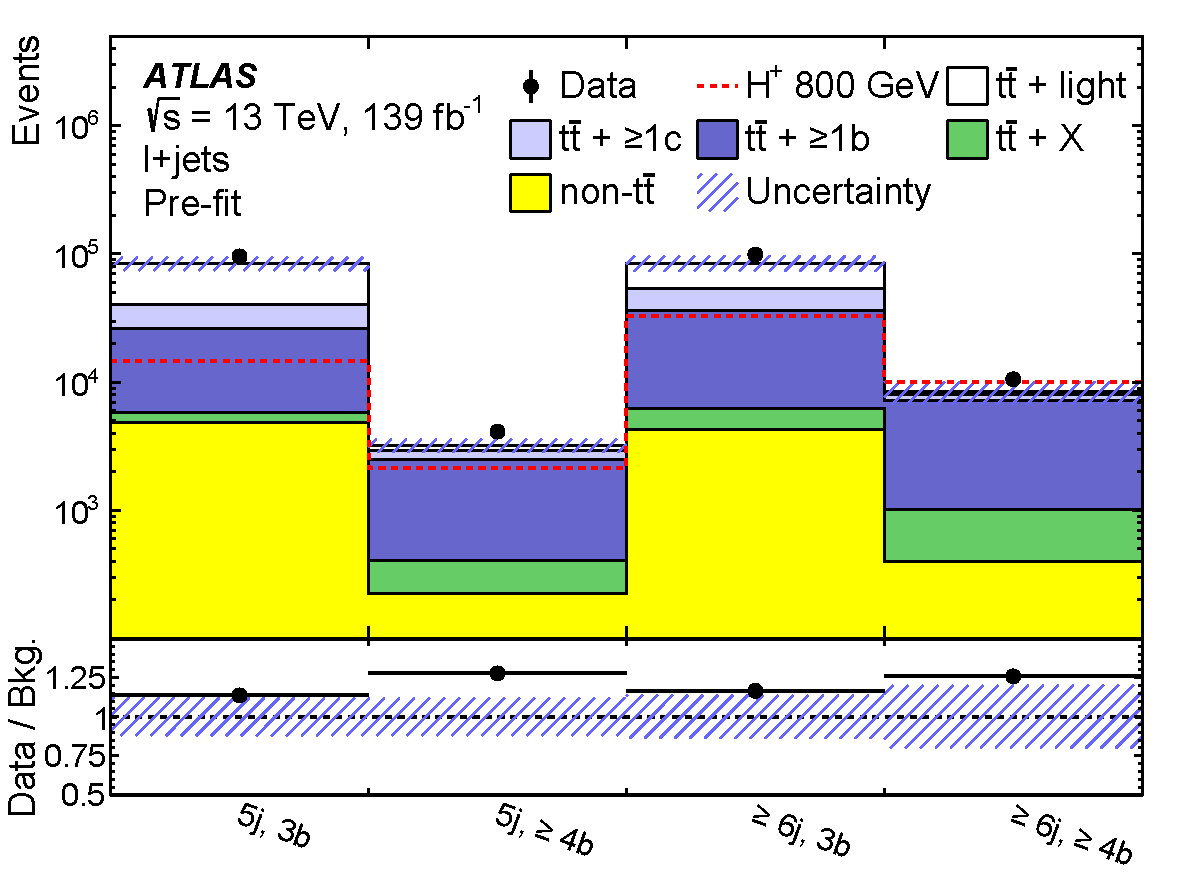
\includegraphics[width = 0.8\textwidth]{HPLUSTB/Fits/Summary.pdf}}\\
    \subfloat[Post-fit]{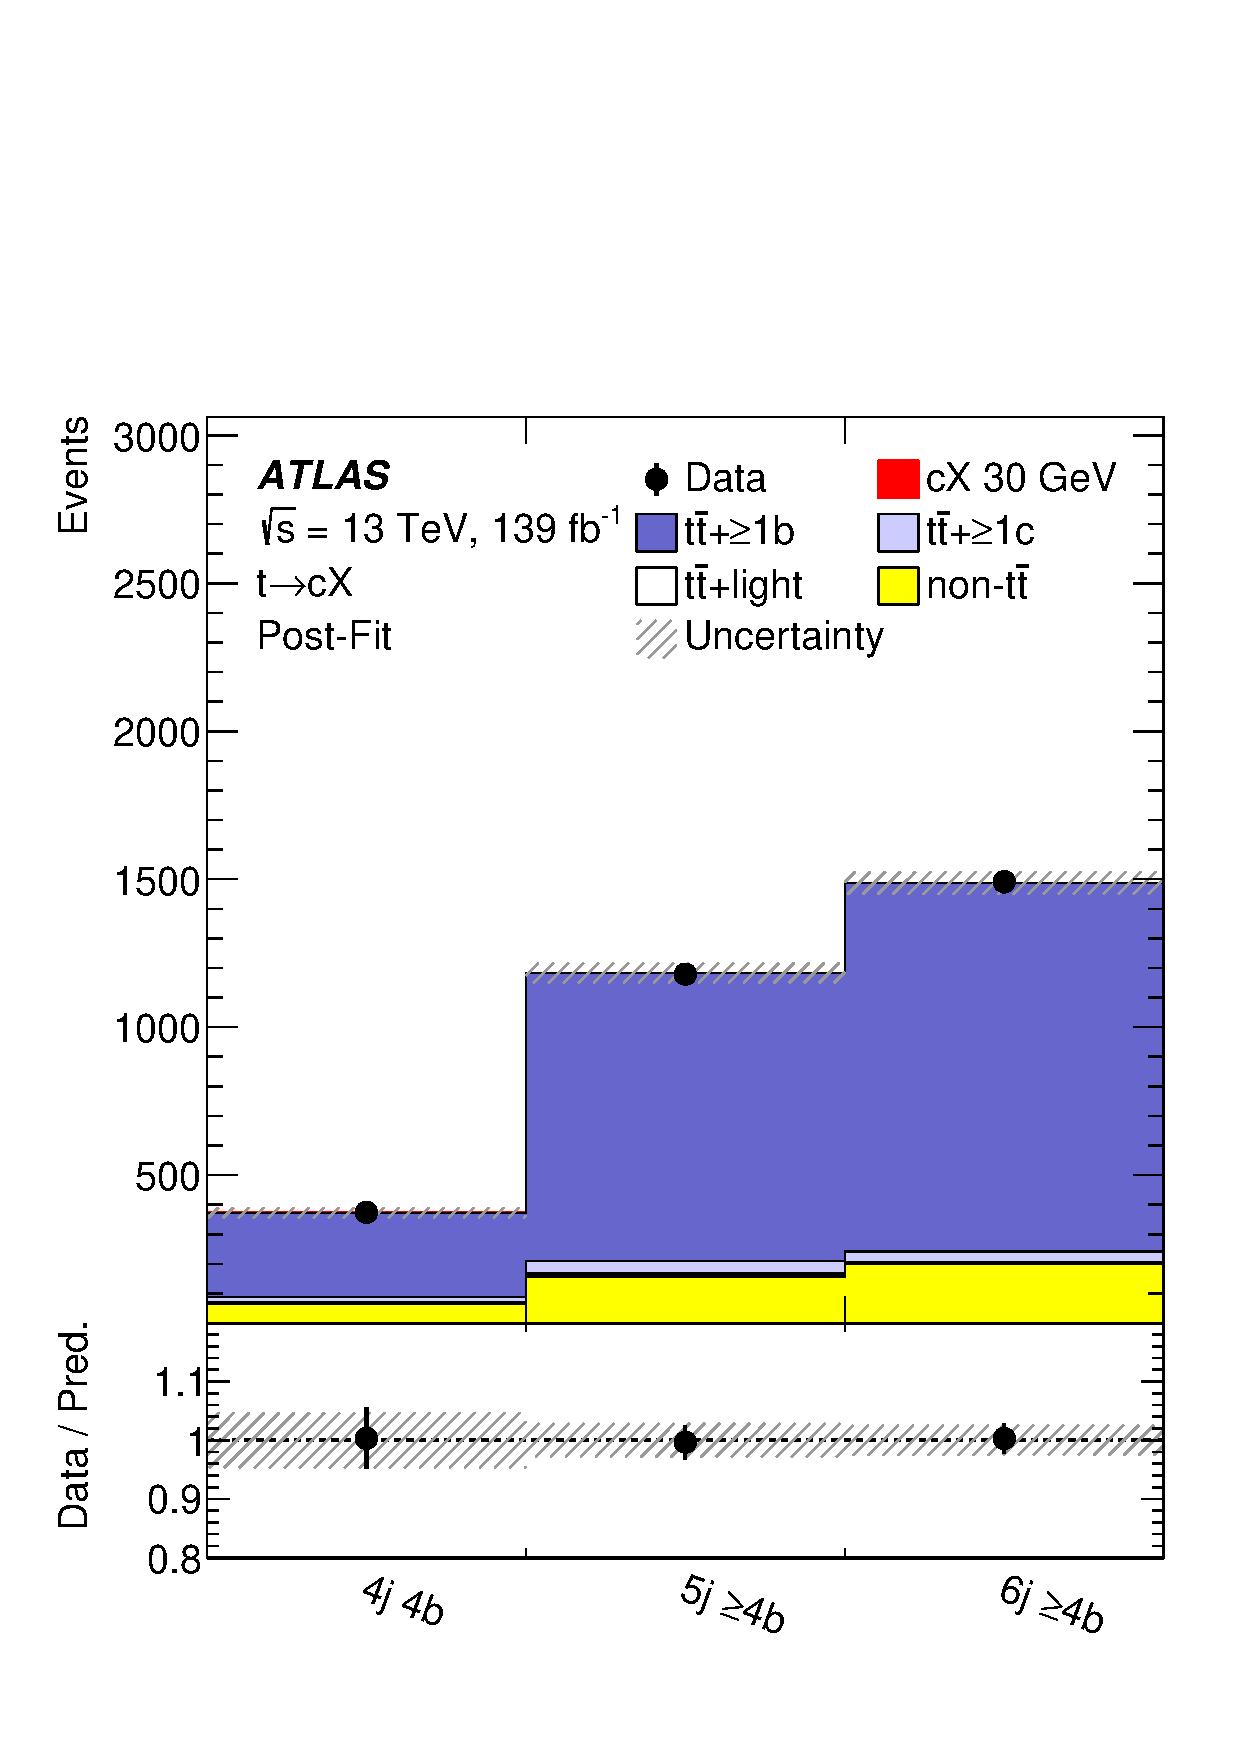
\includegraphics[width = 0.8\textwidth]{HPLUSTB/Fits/Summary_postFit.pdf}}
    \caption{Comparison of predicted and observed event yields before (a) and after (b) the fit in each of the signal regions for the 800~GeV hypothesis. The lower panel displays the ratio of the data to the total prediction and the hatched band shows the uncertainties. The pre-fit yields of a charged Higgs boson with a mass of 800~GeV corresponding to a cross-section of 10~pb are overlaid in red in the figure before the fit.}
    \label{Hplustb:Summaryyieldsplot800}
\end{figure}


\begin{table}[htb]
    \small
    \addtolength{\leftskip} {-2cm} % menja marges
    \addtolength{\rightskip}{-2cm}
    \centering
    \caption{
    Event yields of the $H^+\to tb$ signal and background processes in the four signal regions 
    after the fit to the data under the $H^+$ hypotheses of 200 (top) and 800~GeV (bottom).
    The quoted uncertainties take into account correlations and constraints of the nuisance parameters
    and include both the statistical and systematic uncertainties. Negative correlations among \ttb, \ttc\ and \ttl\ modelling uncertainties can cause the uncertainty on the total yields to be smaller than on individual components. \vspace{0.5cm}
    } 
    \begin{tabular}{l c c c c}
    \toprule\toprule
    \multicolumn{5}{c}{200~GeV $H^+$ hypothesis}  \\
    \midrule \midrule
        & {5j3b} & {5j$\geq$4b} & {$\geq$ 6j3b} & {$\geq$ 6j$\geq$4b}   \\
    \midrule 
  \ttl                  & 45000 $\pm$ 4000 & ~~310 $\pm$ 110 & 32000 $\pm$ 4000 & ~~340 $\pm$ 140  \\ 
  \ttb                  & 29600 $\pm$ 2900 & 2940 $\pm$ 220 & 40200 $\pm$ 3300 & 8000 $\pm$ 500  \\ 
  \ttc                  & 14000 $\pm$ 4000 & ~~440 $\pm$ 140 & 19000 $\pm$ 6000 & 1010 $\pm$ 290  \\ 
  $t\bar{t}$ + $W$        & 110 $\pm$ 15 & ~~3.2 $\pm$ 0.6 & 236 $\pm$ 35 & 16.2 $\pm$ 2.7  \\ 
  $t\bar{t}$ + $Z$        & 300 $\pm$ 40 & 51 $\pm$ 6 & 670 $\pm$ 90 & 174 $\pm$ 23  \\ 
  Single-top $Wt$-channel & 2300 $\pm$ 600 & ~~80 $\pm$ 50 & 1900 $\pm$ 800 & 150 $\pm$ 90  \\
  Single-top $t$-channel & ~~740 $\pm$ 300 & ~~51 $\pm$ 20 & ~~500 $\pm$ 400 & ~~60 $\pm$ 50  \\ 
  Other top-quark sources       & 128 $\pm$ 16 & 17.5 $\pm$ 3.2 & 180 $\pm$ 70 & ~~58 $\pm$ 24 \\ 
  $VV$ \& $V$ + jets      & 1600 $\pm$ 600 & ~~65 $\pm$ 23 & 1600 $\pm$ 600 & 120 $\pm$ 40  \\ 
  $t\bar{t}H$             & 530 $\pm$ 60 & 127 $\pm$ 19 & 1140 $\pm$ 120 & 430 $\pm$ 60  \\ 
\midrule  
$H^+\to tb$                & ~~600 $\pm$ 900 & ~~70 $\pm$ 90 & ~~~~700 $\pm$ 1000 & ~~160 $\pm$ 230  \\ 
\midrule  
  Total                   & 95700 $\pm$ 2900 & 4150 $\pm$ 140 & 98400 $\pm$ 2900 & 10500 $\pm$ 400~~  \\ 
\midrule
  Data                    & 95852             & 4109             & 98929             & 10552    \\
\bottomrule 
\noalign{\vskip 1cm}  
\toprule
\multicolumn{5}{c}{800~GeV $H^+$ hypothesis}   \\
\midrule \midrule
        & {5j3b} & {5j$\geq$4b} & {$\geq$ 6j3b} & {$\geq$ 6j$\geq$4b}   \\
    \midrule 
\ttl                  & 46000 $\pm$ 4000 & ~~330 $\pm$ 120 & 33000 $\pm$ 4000 & ~~500 $\pm$ 200   \\
\ttb                  & 29600 $\pm$ 3100 & 2920 $\pm$ 210 & 41000 $\pm$ 4000 & 8100 $\pm$ 400  \\ 
\ttc                  & 14000 $\pm$ 6000 & ~~440 $\pm$ 190 & 17000 $\pm$ 7000 & ~~870 $\pm$ 330   \\ 
$t\bar{t}$ + $W$        & 108 $\pm$ 15 & ~~3.3 $\pm$ 0.6 & 233 $\pm$ 35 & 16.0 $\pm$ 2.7  \\ 
$t\bar{t}$ + $Z$        & 300 $\pm$ 40 & 50 $\pm$ 7 & 660 $\pm$ 90 & 171 $\pm$ 23  \\ 
Single-top $Wt$-channel & 2000 $\pm$ 500 & ~~56 $\pm$ 33 & 1400 $\pm$ 500 & 100 $\pm$ 60   \\ 
Single-top $t$-channel  & ~~740 $\pm$ 300 & ~~53 $\pm$ 21 & ~~600 $\pm$ 500 & ~~70 $\pm$ 50  \\ 
Other top-quark sources       & 130 $\pm$ 16 & 17.7 $\pm$ 3.2 & 190 $\pm$ 70 & ~~61 $\pm$ 24 \\ 
$VV$ \& $V$ + jets      & 1900 $\pm$ 700 & ~~73 $\pm$ 25 & 1700 $\pm$ 600 & 130 $\pm$ 50   \\ 
$t\bar{t}H$             & 520 $\pm$ 60 & 125 $\pm$ 19 & 1130 $\pm$ 120 & 420 $\pm$ 60 \\ 
\midrule 
$H^+\to tb$                 & ~~30 $\pm$ 80 & ~~~~4 $\pm$ 10 & ~~~~70 $\pm$ 180 & ~~20 $\pm$ 50   \\ 
\midrule
Total                   & 94700 $\pm$ 2800 & 4070 $\pm$ 140 & 97800 $\pm$ 2800 & 10400 $\pm$ 400~~ \\
\midrule
Data                    & 95852             & 4109             & 98929             & 10552 \\
\bottomrule \bottomrule
    \end{tabular}
    \label{Hplustb:postfityields}
\vspace{1cm}
\end{table}

Pre-fit and post-fit distributions of the NN output in the signal regions are shown in Figure~\ref{Hplustb:prepost2005j} to Figure~\ref{Hplustb:prepost8006j} for the different regions and for the 200~GeV and 800~GeV mass hypothesis fits. The agreement between the observed and expected distributions improves after the fit.\\

\begin{figure}[htb]
    \RawFloats
    \centering
    \subfloat[5j3b pre-fit]{\includegraphics[width = 0.5\textwidth]{HPLUSTB/Fits/Hp200/Pre/plot_5jex3bex_NN.pdf}}
    \subfloat[5j3b post-fit]{\includegraphics[width = 0.5\textwidth]{HPLUSTB/Fits/Hp200/Post/plot_5jex3bex_NN.pdf}}\\
    \subfloat[5j$\geq$4b pre-fit]{\includegraphics[width = 0.5\textwidth]{HPLUSTB/Fits/Hp200/Pre/plot_5jex4bin_NN.pdf}}
    \subfloat[5j$\geq$4b post-fit]{\includegraphics[width = 0.5\textwidth]{HPLUSTB/Fits/Hp200/Post/plot_5jex4bin_NN.pdf}}\\
    \caption{Distributions of the NN output in the 5j signal regions before (left) and after (right) the fit for the 200~GeV $H^+$ mass hypothesis. The lower panels display the ratio of the data to the total prediction. The hatched bands show the corresponding uncertainties.
    }
    \label{Hplustb:prepost2005j}
\end{figure}

\begin{figure}[htb]
    \RawFloats
    \centering
    \subfloat[$\geq$6j3b pre-fit]{\includegraphics[width =0.5\textwidth]{HPLUSTB/Fits/Hp200/Pre/plot_6jin3bex_NN.pdf}}
    \subfloat[$\geq$6j3b post-fit]{\includegraphics[width =0.5\textwidth]{HPLUSTB/Fits/Hp200/Post/plot_6jin3bex_NN.pdf}}\\
    \subfloat[$\geq$6j$\geq$4b pre-fit]{\includegraphics[width =0.5\textwidth]{HPLUSTB/Fits/Hp200/Pre/plot_6jin4bin_NN.pdf}}
    \subfloat[$\geq$6j$\geq$4b post-fit]{\includegraphics[width =0.5\textwidth]{HPLUSTB/Fits/Hp200/Post/plot_6jin4bin_NN.pdf}}\\
    \caption{Distributions of the NN output in the $\geq$6j signal regions before (left) and after (right) the fit for the 200~GeV $H^+$ mass hypothesis. The lower panels display the ratio of the data to the total prediction. The hatched bands show the corresponding uncertainties.
    }
    \label{Hplustb:prepost2006j}
\end{figure}

\begin{figure}[htb]
    \RawFloats
    \centering
    \subfloat[5j3b pre-fit]{\includegraphics[width = 0.5\textwidth]{HPLUSTB/Fits/Hp800/Pre/plot_5jex3bex_NN.pdf}}
    \subfloat[5j3b post-fit]{\includegraphics[width = 0.5\textwidth]{HPLUSTB/Fits/Hp800/Post/plot_5jex3bex_NN.pdf}}\\
    \subfloat[5j$\geq$4b pre-fit]{\includegraphics[width = 0.5\textwidth]{HPLUSTB/Fits/Hp800/Pre/plot_5jex4bin_NN.pdf}}
    \subfloat[5j$\geq$4b post-fit]{\includegraphics[width = 0.5\textwidth]{HPLUSTB/Fits/Hp800/Post/plot_5jex4bin_NN.pdf}}\\
    \caption{Distributions of the NN output in the 5j signal regions before (left) and after (right) the fit for the 800~GeV $H^+$ mass hypothesis. The lower panels display the ratio of the data to the total prediction. The hatched bands show the corresponding uncertainties.
    }
    \label{Hplustb:prepost8005j}
\end{figure}

\begin{figure}[htb]
    \RawFloats
    \centering
    \subfloat[$\geq$6j3b pre-fit]{\includegraphics[width = 0.5\textwidth]{HPLUSTB/Fits/Hp800/Pre/plot_6jin3bex_NN.pdf}}
    \subfloat[$\geq$6j3b post-fit]{\includegraphics[width = 0.5\textwidth]{HPLUSTB/Fits/Hp800/Post/plot_6jin3bex_NN.pdf}}\\
    \subfloat[$\geq$6j$\geq$4b pre-fit]{\includegraphics[width = 0.5\textwidth]{HPLUSTB/Fits/Hp800/Pre/plot_6jin4bin_NN.pdf}}
    \subfloat[$\geq$6j$\geq$4b post-fit]{\includegraphics[width = 0.5\textwidth]{HPLUSTB/Fits/Hp800/Post/plot_6jin4bin_NN.pdf}}\\
    \caption{Distributions of the NN output in the $\geq$6j signal regions before (left) and after (right) the fit for the 800~GeV $H^+$ mass hypothesis. The lower panels display the ratio of the data to the total prediction. The hatched bands show the corresponding uncertainties.
    }
    \label{Hplustb:prepost8006j}
\end{figure}
\clearpage

The nuisance parameters and normalisation factors after the fit are different to the original values, as the fit accommodates for normalisation and shape differences between the observed and predicted distributions, which can vary depending on the $H^+$ mass hypothesis\\

The normalisation factors are summarised in Figure~\ref{Hplustb:fittedfactorsvsmass}, and range from 1.33 to 1.36 (0.94 to 1.1) with a typical uncertainty of 0.23 (0.48) for the \ttb\ (\ttc) background, depending on the $H^+$ mass hypothesis fit. Regarding the signal strength, the largest deviation with respect to the \acrshort{SMlabel} hypothesis is observed in the low-mass region, between 225--275~GeV. The deviation is negative and does not represent an evidence of the signal. It is understood as the signal in this mass range is the most similar to the \ttHF\ and results in high anti-correlations with its components in the fit.\\

\begin{figure}[htb]
    \RawFloats
    \centering
    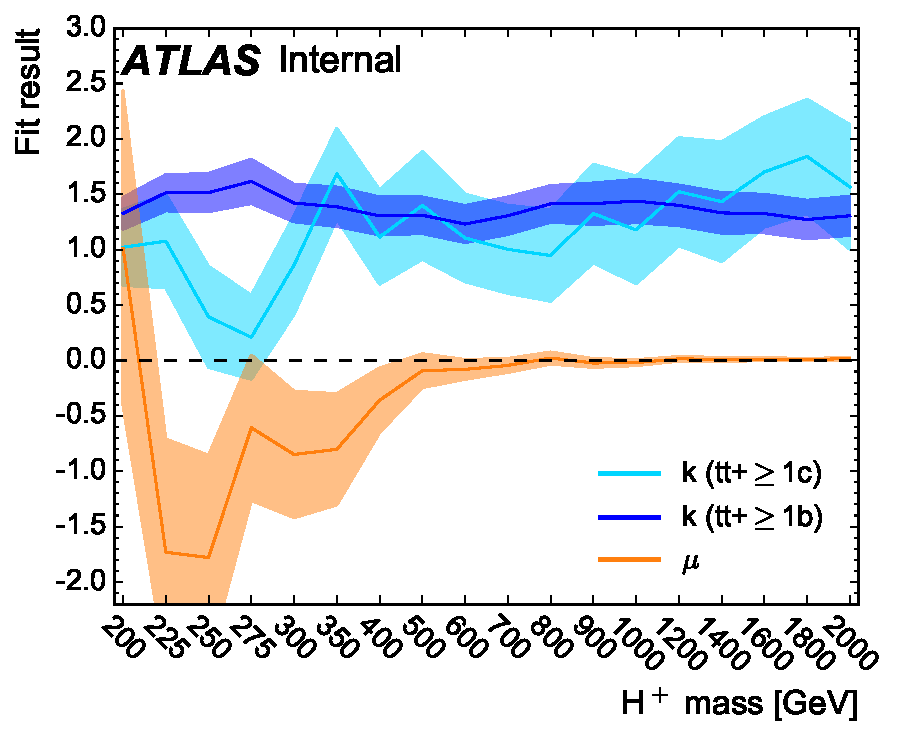
\includegraphics[width = 0.7\textwidth]{HPLUSTB/Fits/Fittedfactors.pdf}
    \caption{Signal strength and the \ttHF\ normalisation factors after the fit as a function of the $H^+$ mass with the corresponding uncertainties. The signal strength is normalised to 1~pb.   
    }
    \label{Hplustb:fittedfactorsvsmass}
\end{figure}


\subsection{Dominant uncertainties}

The total uncertainty of the fit is dominated by systematic uncertainties. The different sources are ranked by the impact on the signal strength in terms of its shift from the default result $\Delta\mu$, evaluated in separate fits where the associated nuisance parameters are fixed to $\hat{\theta}\pm\Delta\hat{\theta}$. The parameter $\hat{\theta}$ is the best fit value of the given nuisance parameter, while $\Delta\hat{\theta}$ is the corresponding one standard deviation.\\

Figure~\ref{Hplustb:ranking200800} lists the 20 top ranked nuisance parameters of the 200 and 800~GeV signal hypothesis fits. The upper axis represents the scale for the pre-fit and post-fit impact on $\mu$. The pre-fit (post-fit) impact is given as $\theta \pm \Delta\theta (\hat{\theta} \pm \Delta\hat{\theta})$, with $\Delta\theta$ ($\Delta\hat{\theta}$) being the pre-fit (post-fit) uncertainties. The post-fit value of $\Delta\hat{\theta}$ is typically smaller than the one standard deviation prior $\Delta\theta$, due to constraints from the fit to data. The pre-fit and post-fit impacts are shown as empty and filled rectangles, respectively. The lower axis indicates the scale of the pull of the nuisance parameter defined as $\frac{\hat{\theta} -\theta_0}{\Delta\theta}$ with $\theta_0$ being he nominal pre-fit value. The pulls are indicated as black points with their respective error bar while the background normalisations ($k$) and the single-bin statistical uncertainties ($\gamma$) are drawn directly, with $\theta_0=0$ and without the pre-fit impact as it is not properly defined.

\begin{figure}[tb]
    \RawFloats
    \centering
    \subfloat[200~GeV hypothesis fit]{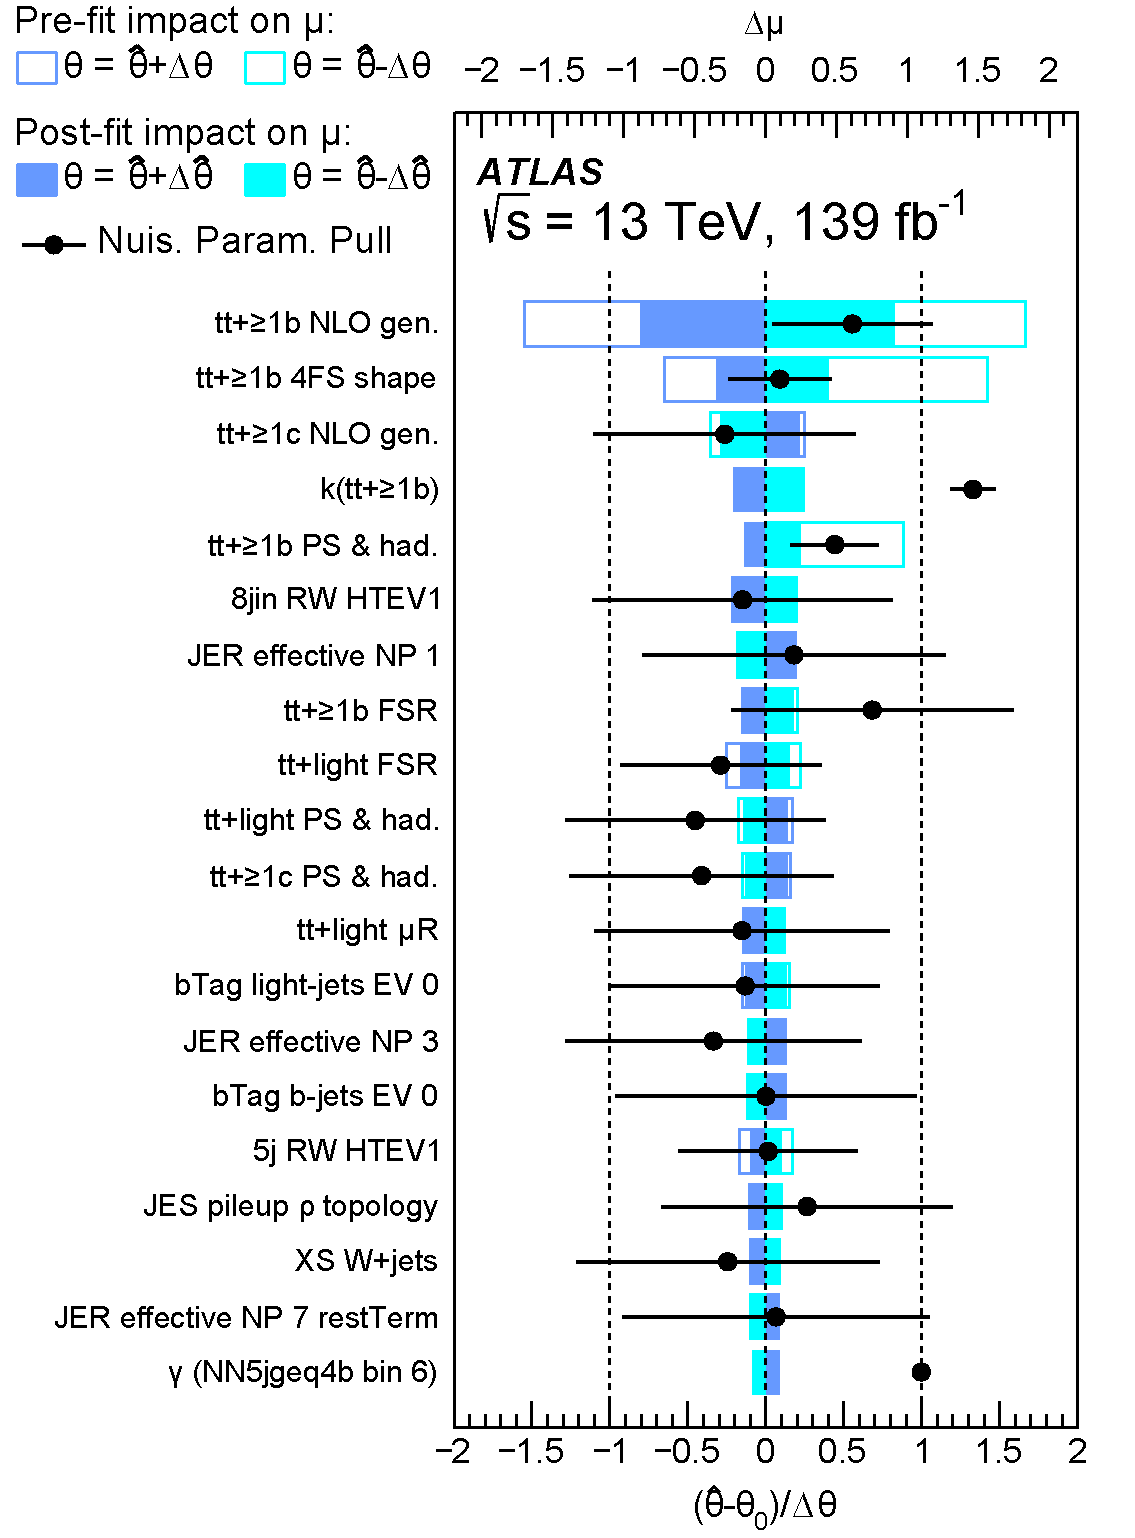
\includegraphics[width = 0.45\textwidth]{HPLUSTB/Fits/Ranking200.pdf}}
    \subfloat[800~GeV hypothesis fit]{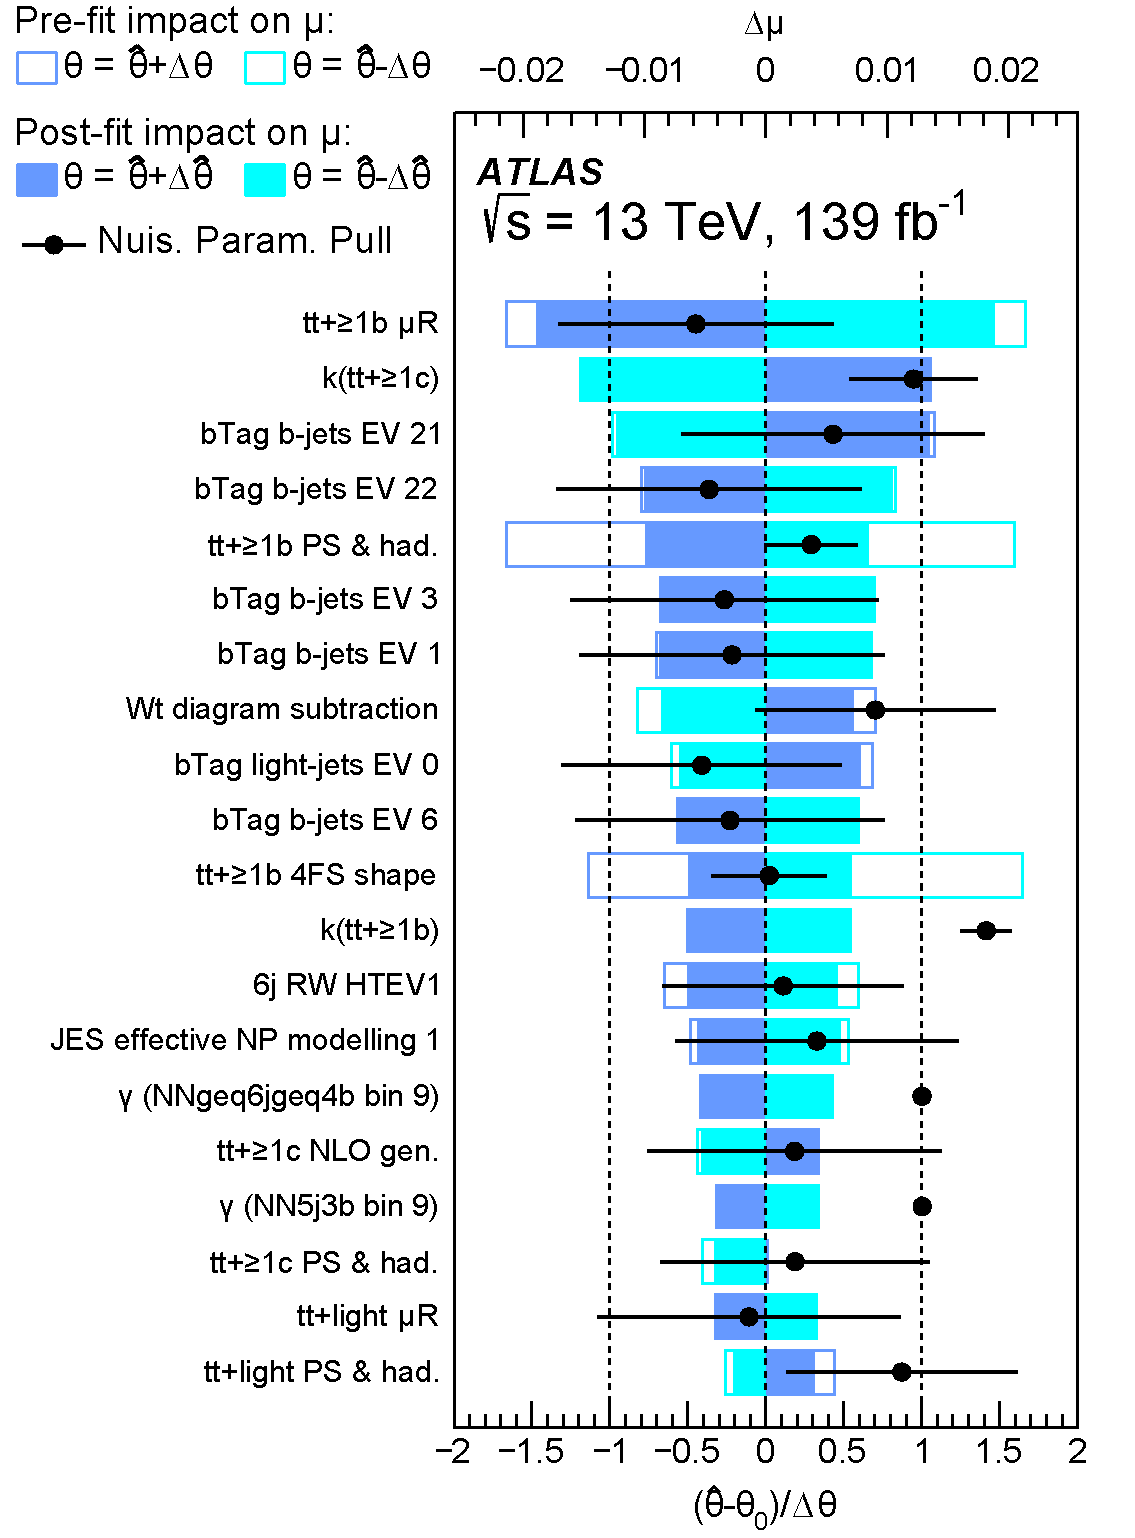
\includegraphics[width = 0.45\textwidth]{HPLUSTB/Fits/Ranking800.pdf}}
    \caption{Ranking of the 20 systematic uncertainties with the largest impact on $\mu$ for the fit performed with the 200 GeV (a) and 800 GeV (b) signal hypotheses. The empty (filled) rectangles correspond
    to the pre-fit (post-fit) impact on $\mu$. The black points represent the post-fit pulls of the nuisance parameters relative to the nominal values, $\theta_0$. Normalisation factors ($k$) and statistical uncertainties ($\gamma$) are shown pulled with respect 1.
    }
    \label{Hplustb:ranking200800}
\end{figure}

The ranking of the uncertainties vary depending on the mass hypotheses. The five highest-ranked nuisance parameters of the 200~GeV signal hypothesis fit are all associated to the $\ttbar+$$\geq$1$b/c$, where the two dominant systematic uncertainties are from the \ttb\ NLO matching (retrieved from the comparison of \MGMCatNLOPYTHIA~8 and \POWHEGPYTHIA~8) and the 4FS \ttb\ (from the comparison of 4FS and 5FS). Besides the \ttbar\ modelling, jet energy resolution and $b$-tagging nuisance parameters appear in the ranking, which have a very small impact in comparison. For the 800~GeV signal hypothesis fit, six $b$-tagging uncertainty components show up in the first 10, and the two top uncertainties are from the \ttb\ renormalisation scale (retrieved varying $\mu_R$) and $k(\ttc)$.\\

Table~\ref{Hplustb:rankingbreak} shows the impact on the signal strength evaluated in groups of systematic uncertainty sources for the 200 and 800~GeV signal hypothesis fits. The total uncertainty is dominated by the systematic uncertainties, with the \ttb\ modelling dominating for both masses. For the 800~GeV fit, the $b$-tagging related uncertainties play also a leading role. For the 200~GeV fit, the sub-leading uncertainties are related to the modelling of \ttc, \ttl\ or jets.\\

\begin{table}[htb]
    \caption{
      Summary of the statistical and systematic uncertainties on 
      $\mu$ for the 200 and 800~GeV signal hypothesis fits. Due to correlations between the different sources of uncertainty, the total systematic uncertainty can be different from the sum in quadrature of the individual sources. The normalisation factors for both \ttb\ and \ttc\ are included in the statistical component.}
    \begin{center}
    \begin{tabular}{l c c}
    \toprule\toprule
    Uncertainty source   & $\Delta\mu(H^+_{200})$ [pb] & $\Delta\mu(H^+_{800})$ [pb] \\
    \midrule \midrule
    \ttb\ modelling                            &  1.01   &  0.025   \\
    Jet energy scale and resolution            &  0.35   &  0.009  \\
    \ttc\ modelling                            &  0.32   &  0.006   \\ %0.0039  \\
    Jet flavour tagging                        &  0.20   &  0.025   \\
    Reweighting                                &  0.22   &  0.007   \\ %0.0066  \\
    \ttl\ modelling                          &  0.33   &  0.009   \\ % 0.0091  \\
    Other background modelling                 &  0.19   &  0.011   \\
    MC statistics                              &  0.11   &  0.008   \\ % 0.0081  \\
    JVT, pile-up modelling                     &  <0.01~~   &  0.001   \\ %0.046  &  0.0022  \\
    Luminosity                                 &  <0.01~~  &  0.002   \\ %0.0022  \\
    Lepton ID, isolation, trigger, \MET        &  <0.01~~  &  <0.001~~  \\ %0.00090 
    $H^+$ modelling                          &  0.05   &  0.002    \\ %0.035 & 0.0016  \\ 
    \midrule
    Total systematic uncertainty               &  1.35   &  0.049    \\ % 0.0499   \\
    \midrule
    \ttb\ normalisation                      &  0.23   &  0.007   \\ %0.0077   \\
    \ttc\ normalisation                      &  ~~0.045  &  0.015   \\
    \midrule
    Total statistical uncertainty              &  0.43   &  0.025   \\ %0.424999 0.025027
    \midrule \midrule
    Total uncertainty                          &  1.42   &  0.055   \\ %1.36089 0.0543417
    \bottomrule \bottomrule
  \end{tabular}
  \end{center}
  \label{Hplustb:rankingbreak}
  \end{table}
  
\clearpage

\section{Exclusion limits}

No significant excess above the expected \acrshort{MClabel} background is observed in all the $H^+$ mass range tested, hence upper limits on the signal production are derived as a function of the $H^+$ mass.\\

Figure~\ref{Hplustb:xseclimits} shows the 95\% confidence level (CL) upper limits on $\sigma(pp\to tbH^+)\times$B$(H^+ \to tb)$ obtained using the CL$_\text{S}$ method~\cite{Cowan_2011}. Two different predictions corresponding to the hMSSM model with $\tan\beta=0.5$ or 1 are shown without uncertainties. The observed (expected) limits range from $\sigma$~$\times$~B = 3.6 (2.6)~pb at $m_{H^+}= 200$~GeV to $\sigma$~$\times$~B = 0.036 (0.019)~pb at $m_{H^+}= 2$~TeV. Compared to the previous \acrshort{ATLASlabel} search with 36~fb$^{-1}$~\cite{ATLASHptb2018}, the observed $\sigma$~$\times$~B limits improved by 5\% to 70\%, depending on the $H^+$ mass, apart from the lowest one.

\begin{figure}[htb]
    \RawFloats
    \centering
    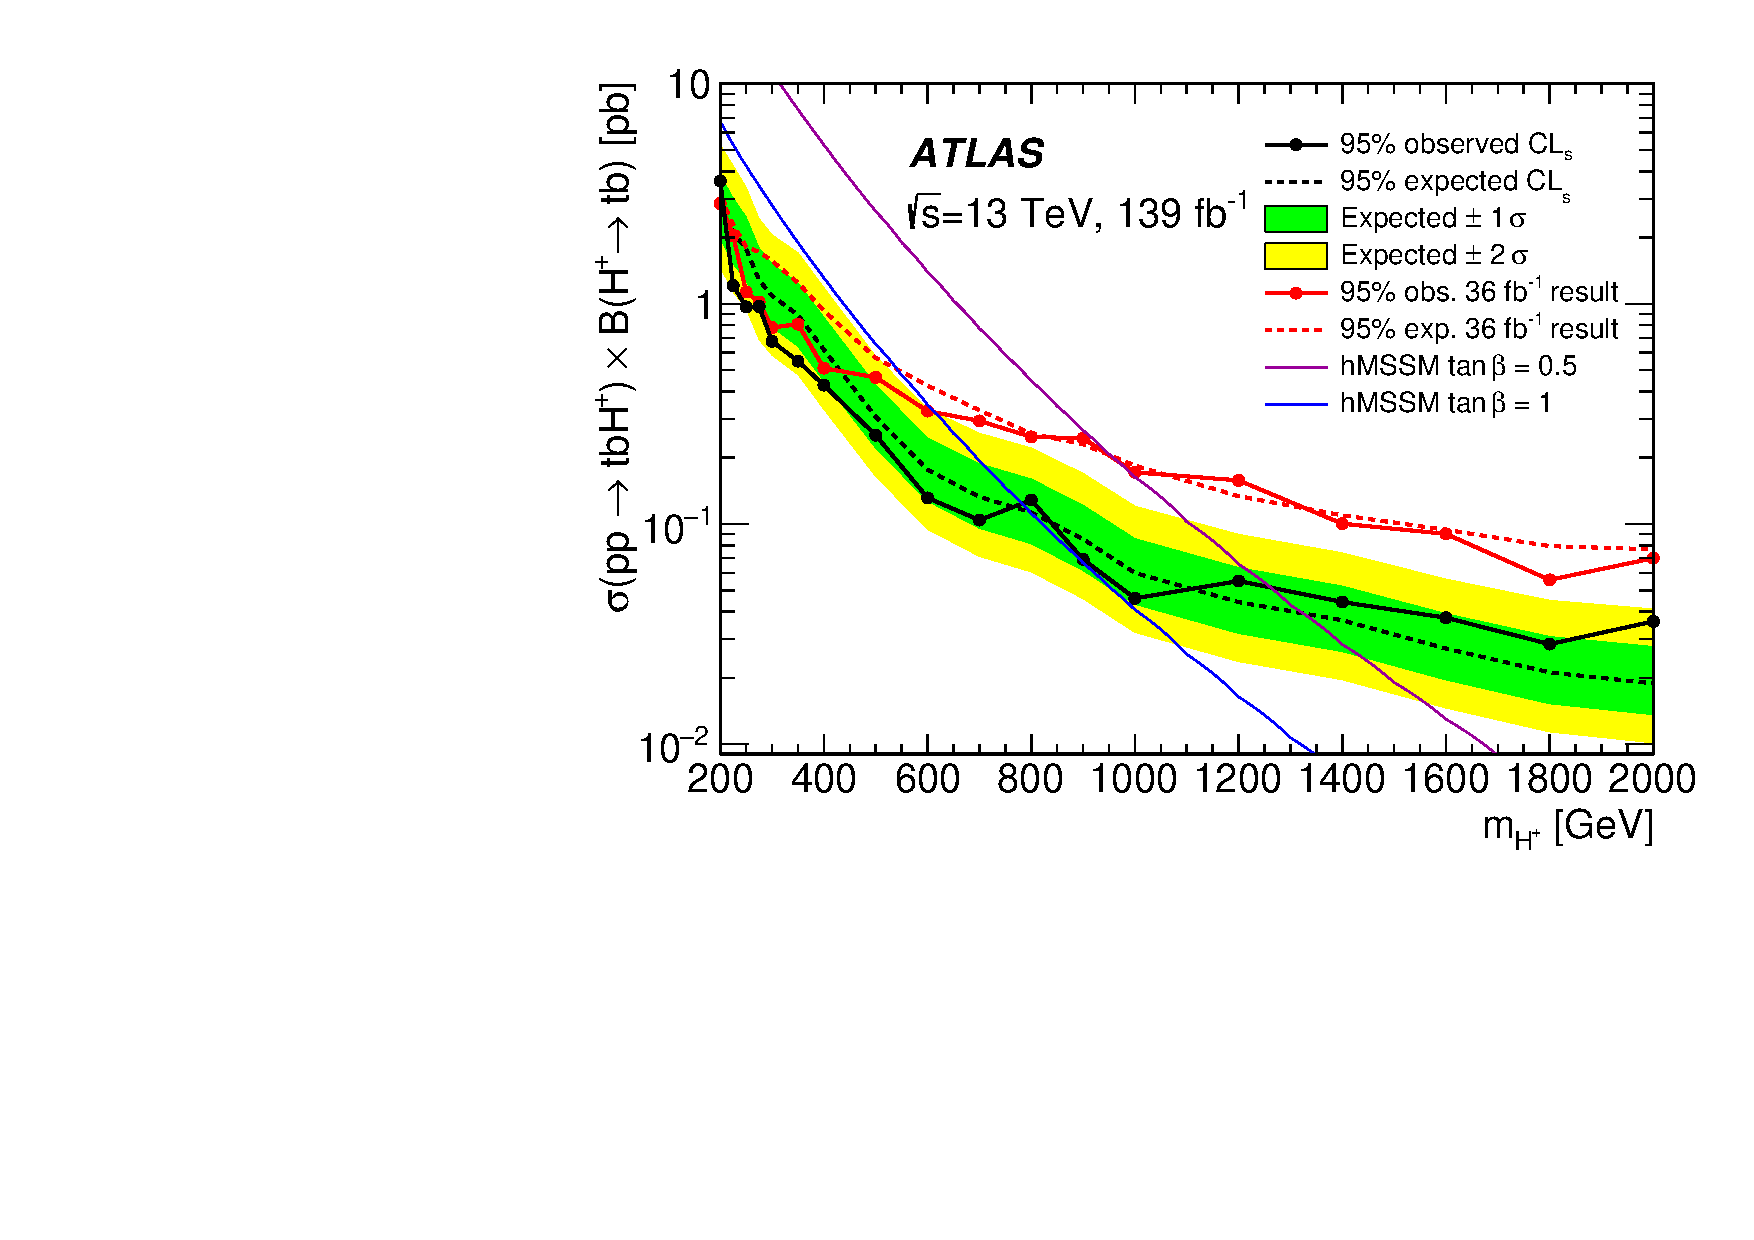
\includegraphics[width = 0.9\textwidth]{HPLUSTB/Fits/Limit_xsec_4FSsysSonly.pdf}
    \caption{Observed and expected upper limits for the production of $H^+\to tb$ in association with
    a top quark and a bottom quark. The bands surrounding the expected limit show the 68\% and
    95\% confidence intervals. The red lines show the observed and expected 95\% CL exclusion limits
    obtained with the 36 fb$^{-1}$ data sample~\cite{ATLASHptb2018}. Theory predictions are shown for two representative values of $\tan\beta$ in the hMSSM benchmark scenario. Uncertainties in the predicted $H^+$ cross-sections or branching ratios are not considered.}
    \label{Hplustb:xseclimits}
\end{figure}

The obtained $H^+\to tb$ production upper limits results are model independent, and therefore can be interpreted in the context of various \acrshort{BSMlabel} theories as long as the topology and kinematics of the targeted channel remains equivalent. Figure~\ref{Hplustb:exclusionstanb} shows 95\% CL exclusion limits set on the $\tan\beta$ parameter as a function of $m_{H^+}$ for various benchmark scenarios in the MSSM. It is the first time that they are shown for all $\text{M}^{125}_\text{h}$ available scenarios using the $H^+\to tb$ channel.\\

In the hMSSM framework, effective couplings of the lighter Higgs boson to the top quark, bottom quark and vector bosons are derived from fits to LHC data on the production and decay rates of the observed Higgs boson, including the limits from the search for heavier neutral and charged Higgs boson states. The $\text{M}^{125}_\text{h}$ scenario is the first, with relatively heavy superparticles so the couplings, $\text{M}^{125}_\text{h}$($\tilde{\chi}$), $\text{M}^{125}_{\text{h}_1}$($\tilde{\tau}$), $\text{M}^{125}_\text{h}$(alignment) and $\text{M}^{125}_\text{h}$(CPV) scenarios also feature a scalar particle with mass and couplings compatible with those of the observed Higgs boson, and force a significant portion of their parameter space to be compatible with the limits from searches for supersymmetric particles. In the $\text{M}^{125}_\text{h}$ scenario, all supersymmetric particles are relatively heavy and the decays of the MSSM Higgs bosons are essentially unaffected, whereas the $\text{M}^{125}_\text{h}$($\tilde{\chi}$) and $\text{M}^{125}_{\text{h}_1}$($\tilde{\tau}$) models include either light charginos and neutralinos or light staus, respectively. In both cases a charged Higgs boson of sufficiently high mass is allowed to decay into the supersymmetric particles. Finally, the value of $\tan\beta$ in both the $\text{M}^{125}_\text{h}$(alignment) scenario, characterised by one of the two neutral CP-even scalars having couplings like those of the SM Higgs boson, and the $\text{M}^{125}_\text{h}$(CPV) scenario, which includes CP violation in the Higgs sector, is already constrained to be in the 1--20 range by previous searches at the \acrshort{LHClabel}~\cite{PhysRevD.91.075015}.\\

Uncertainties in the predicted $H^+$ cross-sections or branching ratios are not included in the limits. For all scenarios except the hMSSM, Higgs boson masses and mixing (and effective Yukawa couplings) have been calculated with the code FeynHiggs~\cite{Heinemeyer_2000,Heinemeyer_1999,Degrassi_2003,Hahn_2014,Frank_2007,Bahl_2016,Bahl_2018}. Whereas in the hMSSM the branching ratios are computed solely with HDECAY~\cite{Djouadi_2019,Djouadi_1998}, all other scenarios combine the most precise results of FeynHiggs, HDECAY and PROPHECY4f~\cite{Bredenstein_2006,Bredenstein_2007}.\\

In the context of these scenarios, $\tan\beta$ values below 1 are observed to be excluded at 95\% CL for $H^+$ masses between 200 and $\sim$790 GeV. High values of $\tan\beta$ between 34 and 60 are excluded in a similar mass range in the hMSSM and $\text{M}^{125}_\text{h}$($\tilde{\chi}$) models. The most stringent limit, $\tan\beta$ < 2.1 excluded at 95\% CL, is set for the $H^+$ mass hypothesis of 225 GeV in the hMSSM and for the 250 GeV $H^+$ mass hypothesis in the different $\text{M}^{125}_\text{h}$ models. The low $\tan\beta$ and high $H^+$ mass parameter space was not excluded by any other analysis before, while the high $\tan\beta$ was already excluded by the \acrshort{ATLASlabel} $H^+\to\tau\nu$ search~\cite{Hplustaunu16}.\\

Compared to previous results of the same search channel~\cite{ATLASHptb2018}, this analysis excludes a broader region of large $\tan\beta$. Additionally, an extended region of low $\tan\beta$ and low and high $H^+$ masses is also excluded.

\begin{figure}[htb]
    \RawFloats
    \centering
       \subfloat[]
       {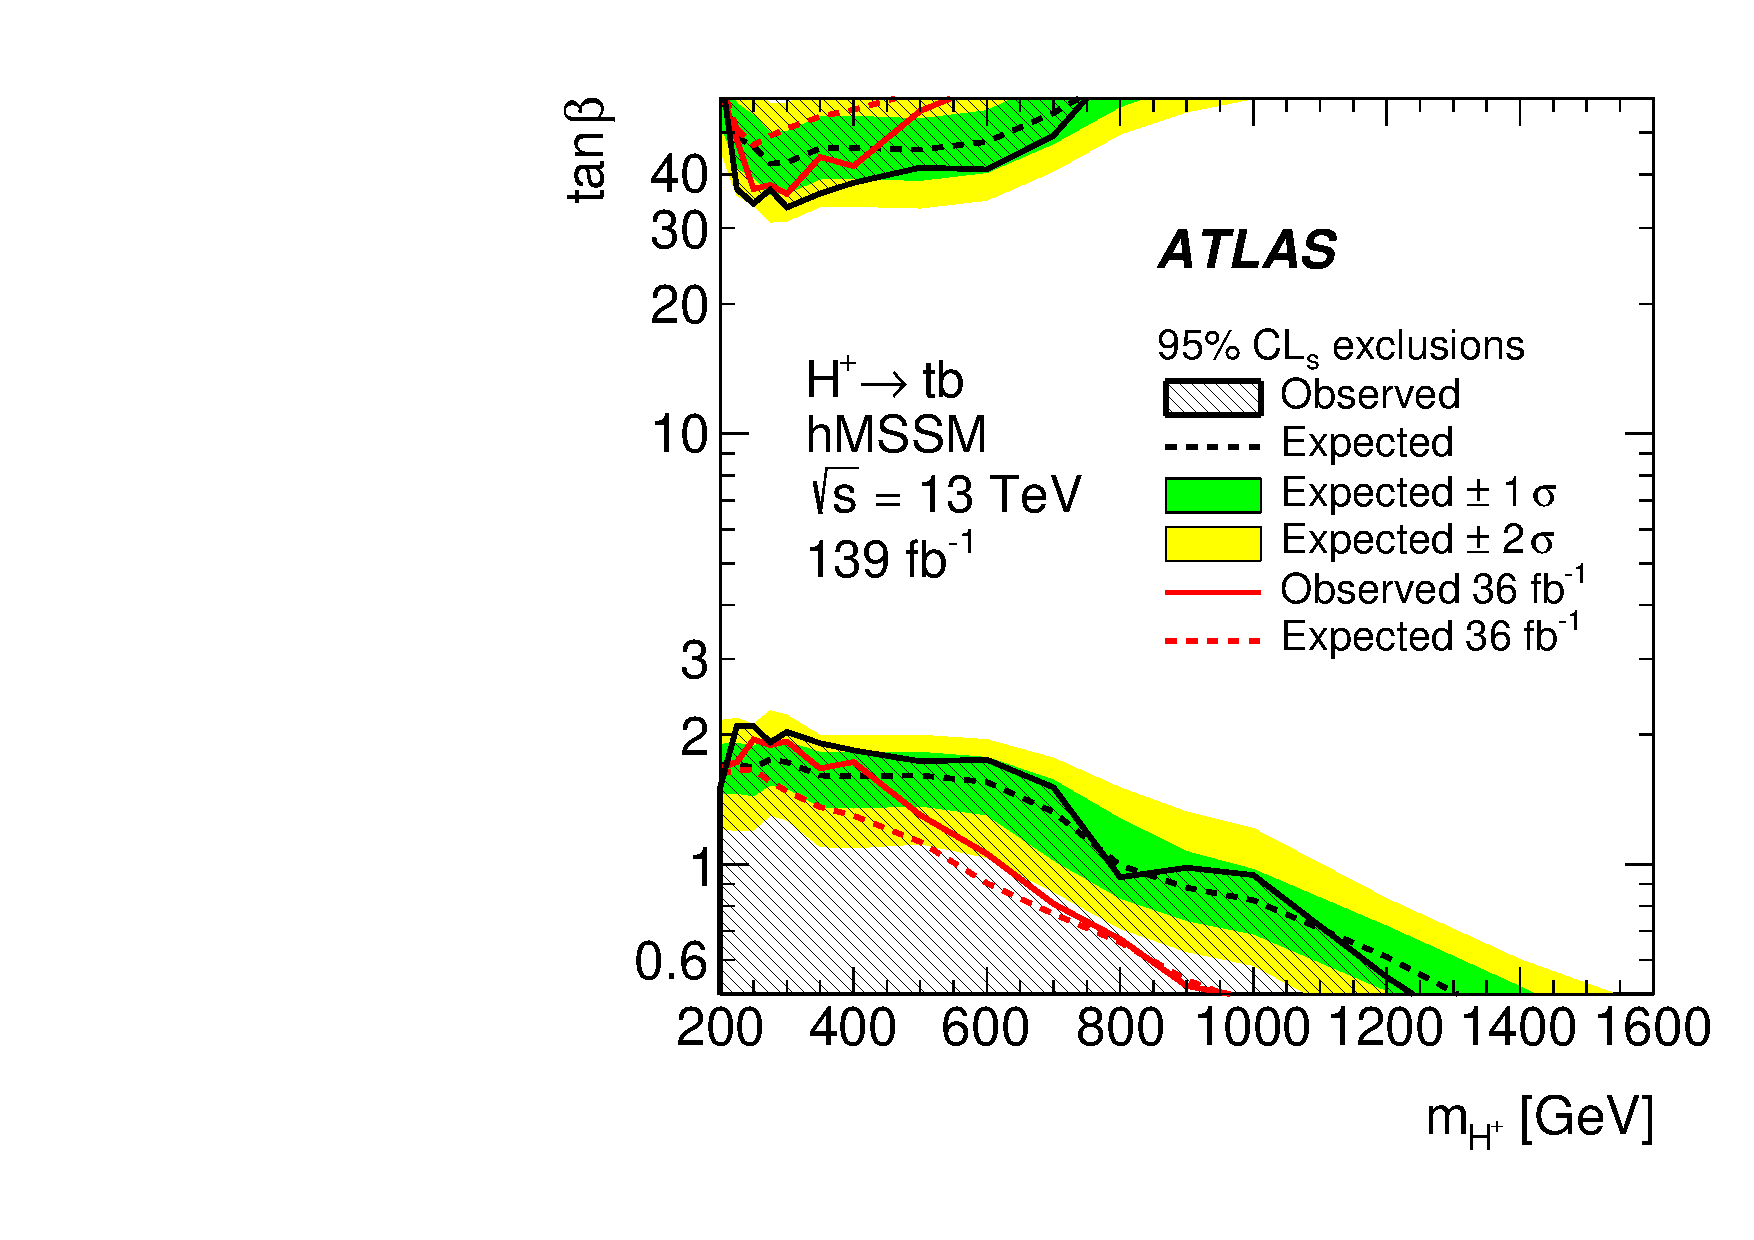
\includegraphics[width = 0.45\textwidth]{HPLUSTB/Fits/Exclusionplot_4FSS_hmssm_tb.pdf}} 
       \subfloat[]
       {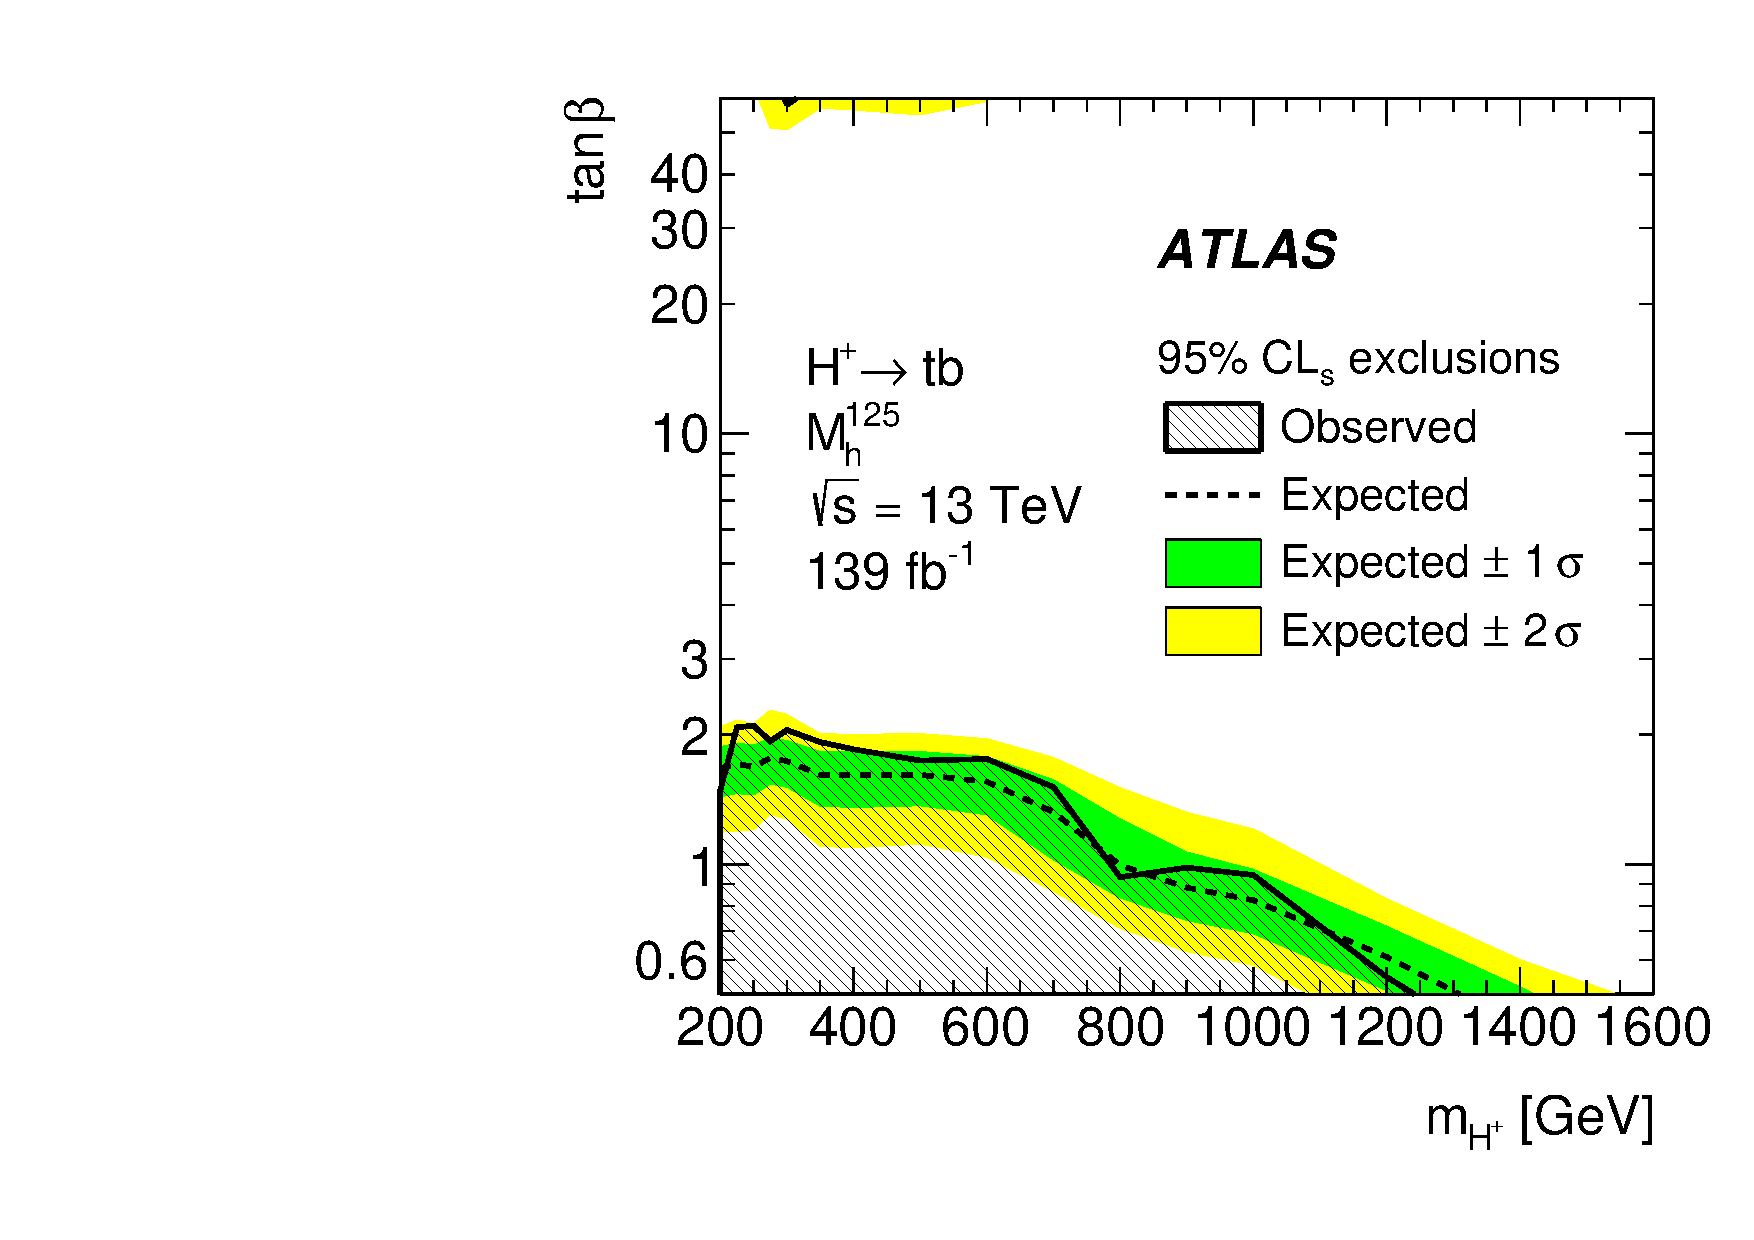
\includegraphics[width = 0.45\textwidth]{HPLUSTB/Fits/Exclusionplot_4FSS_mh125_tb.pdf}} \\
       \subfloat[]
       {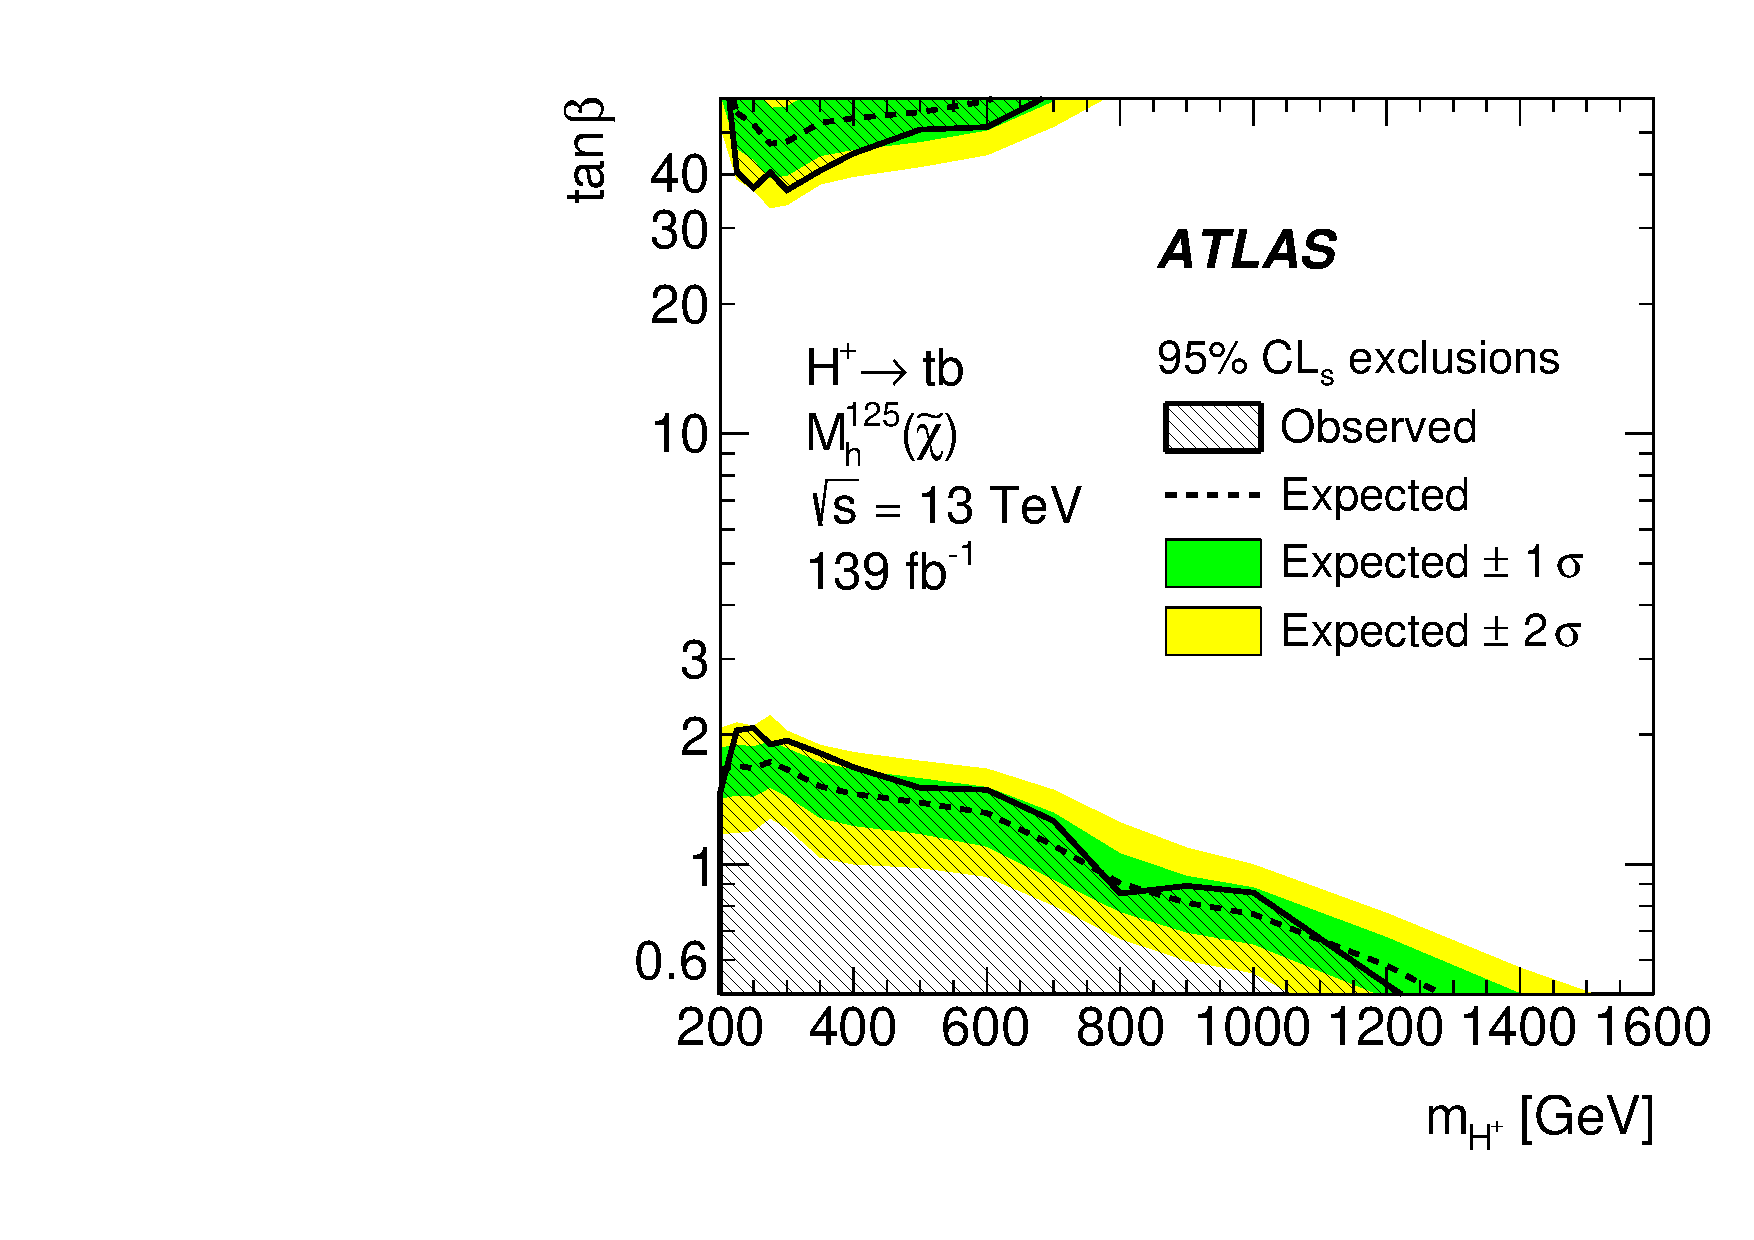
\includegraphics[width = 0.45\textwidth]{HPLUSTB/Fits/Exclusionplot_4FSS_mh125_lc_tb.pdf}}
       \subfloat[]
       {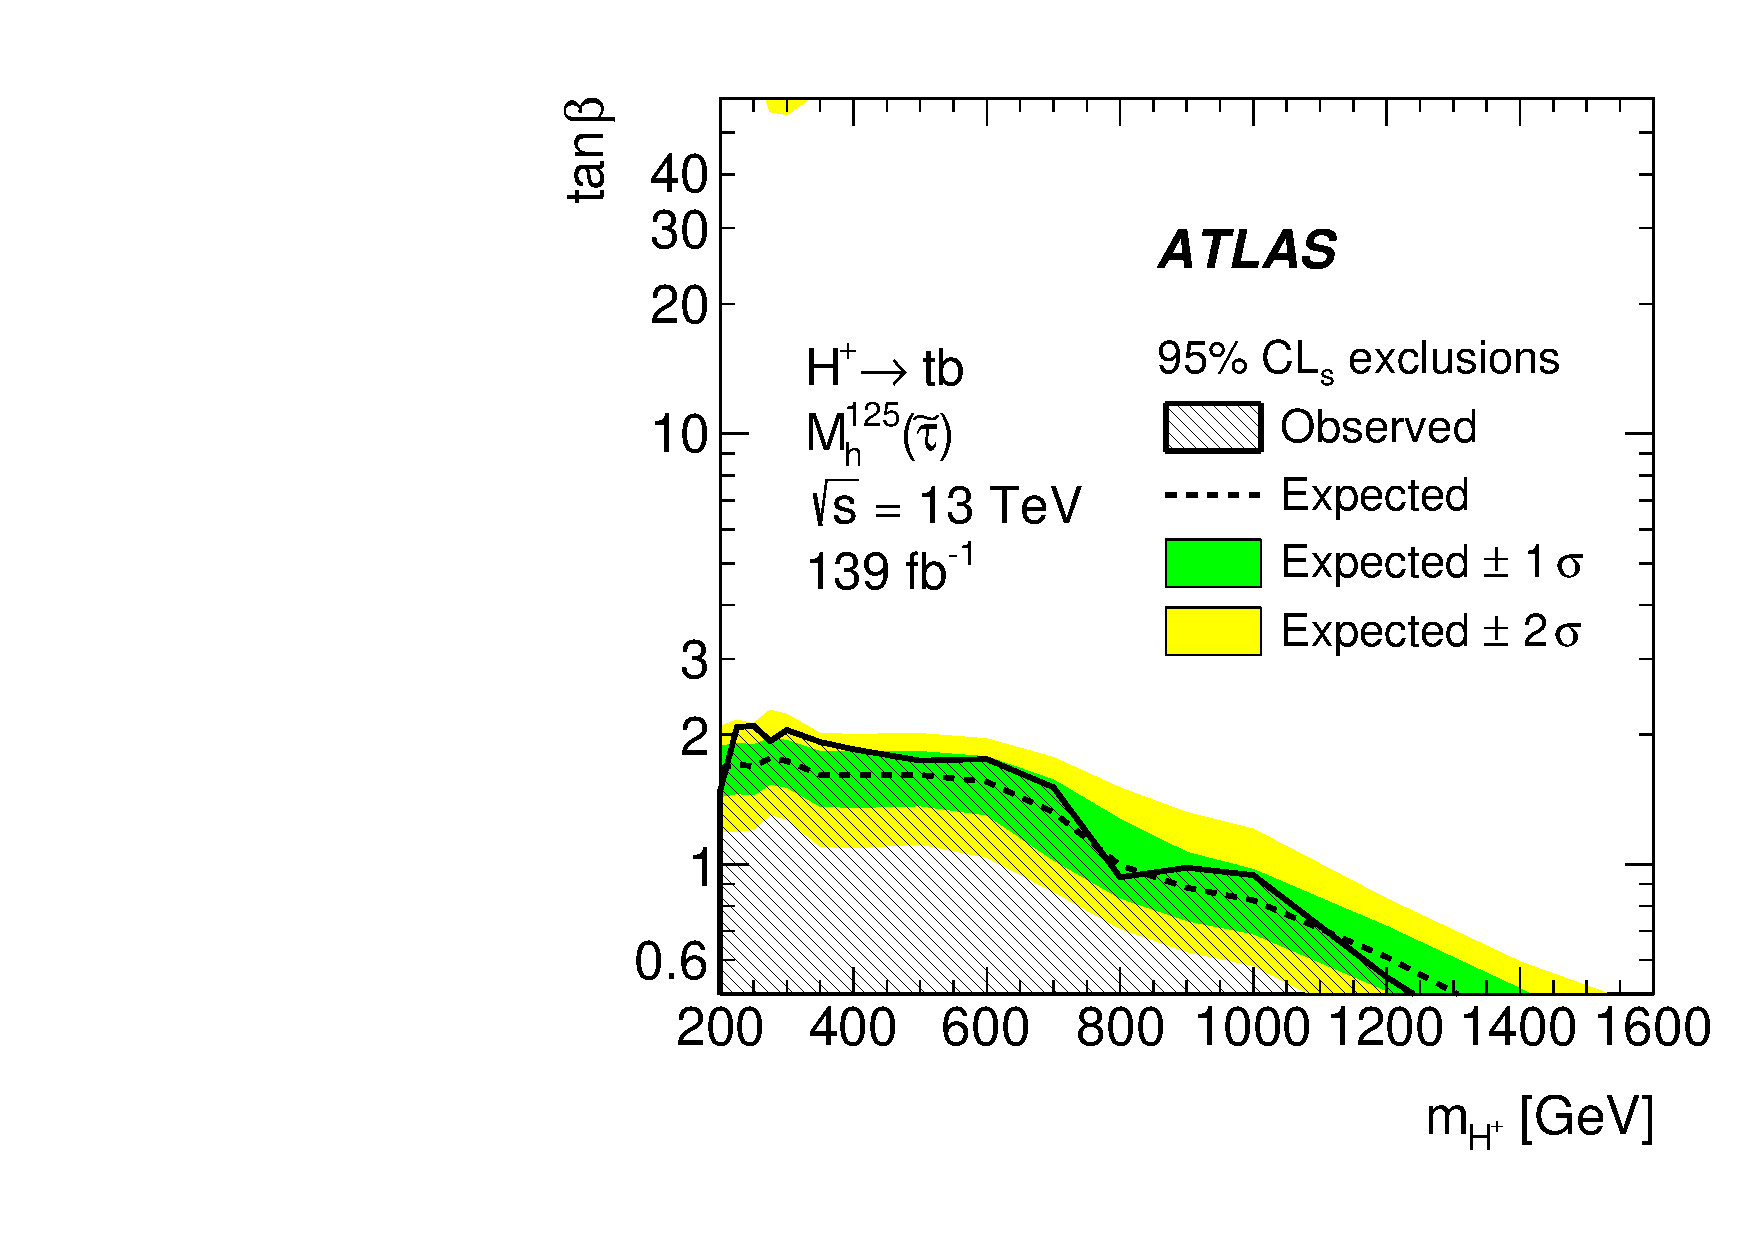
\includegraphics[width = 0.45\textwidth]{HPLUSTB/Fits/Exclusionplot_4FSS_mh125_ls_tb.pdf}} \\
       \subfloat[]
       {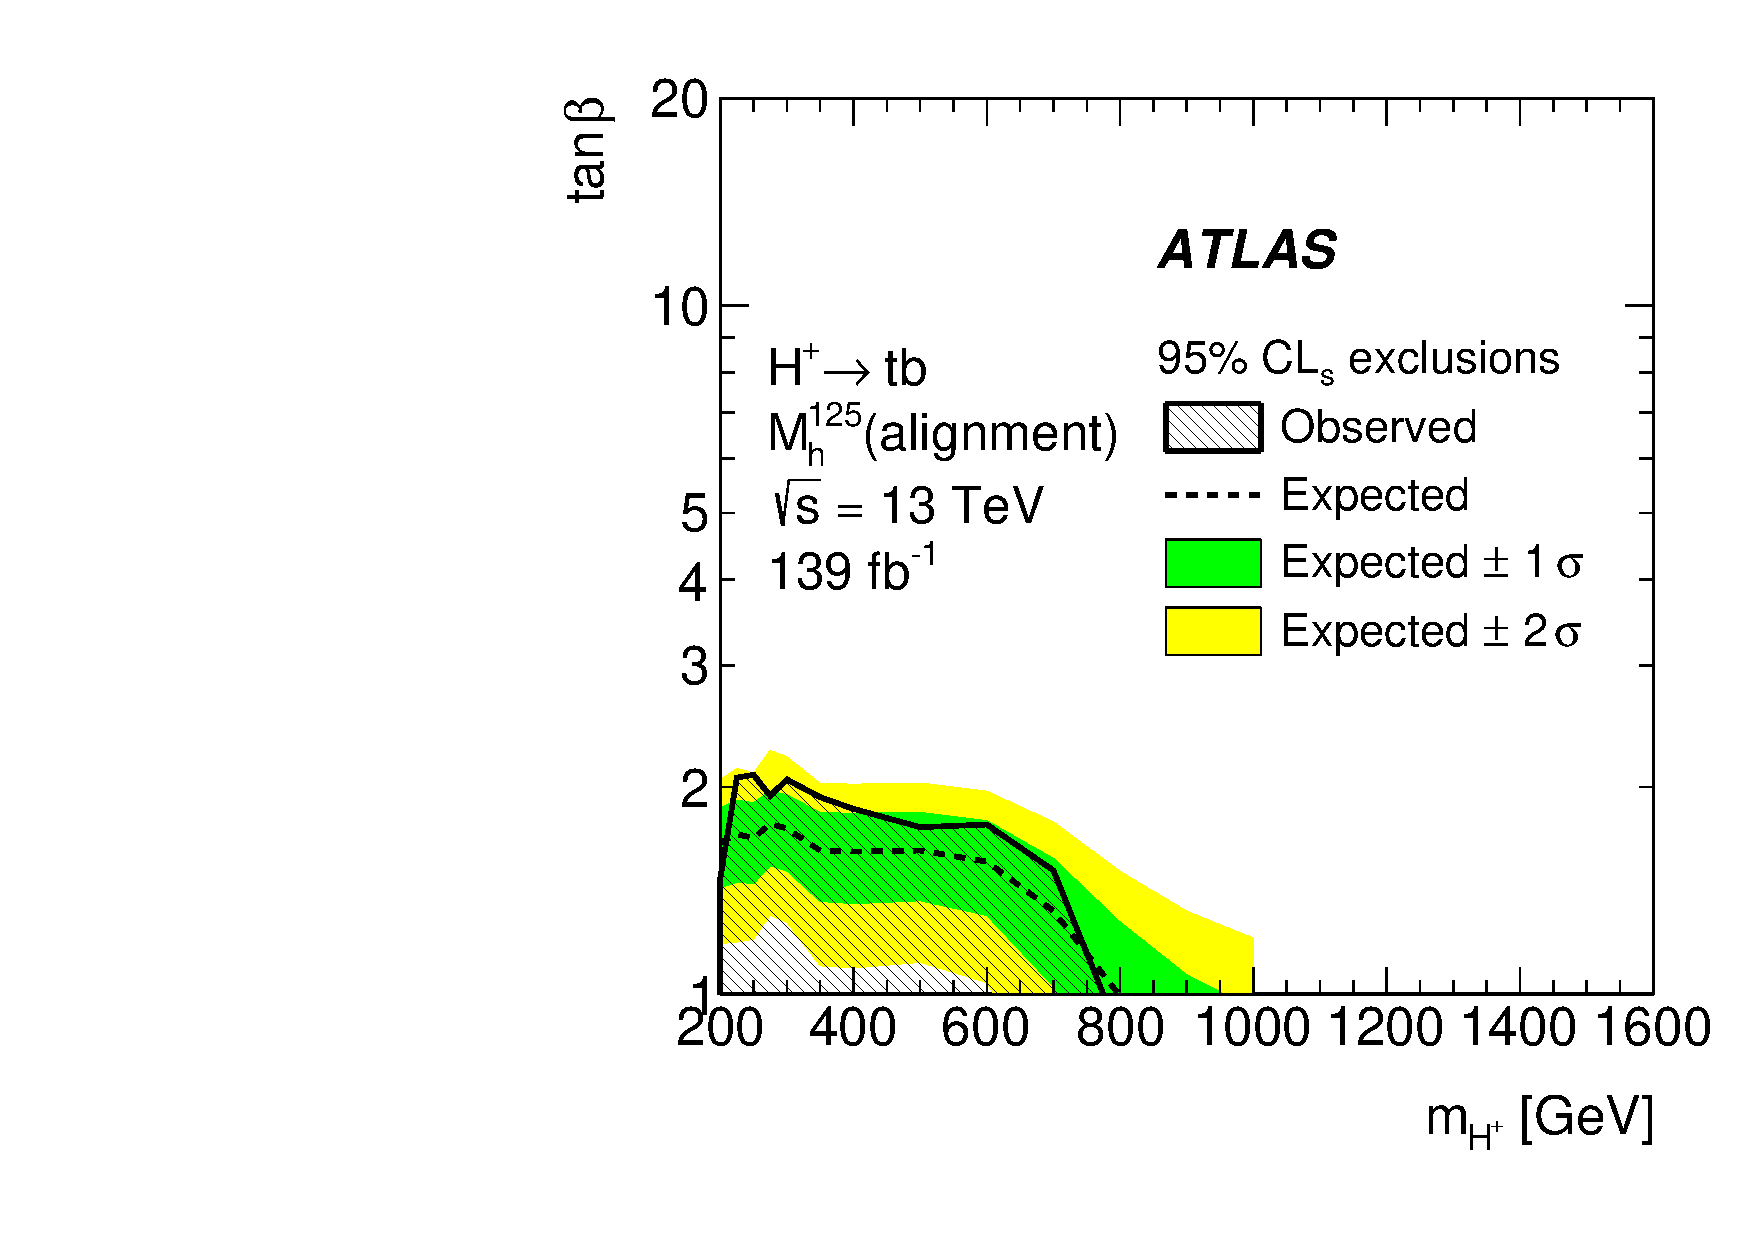
\includegraphics[width = 0.45\textwidth]{HPLUSTB/Fits/Exclusionplot_4FSS_mh125_align_tb.pdf}}
       \subfloat[]
       {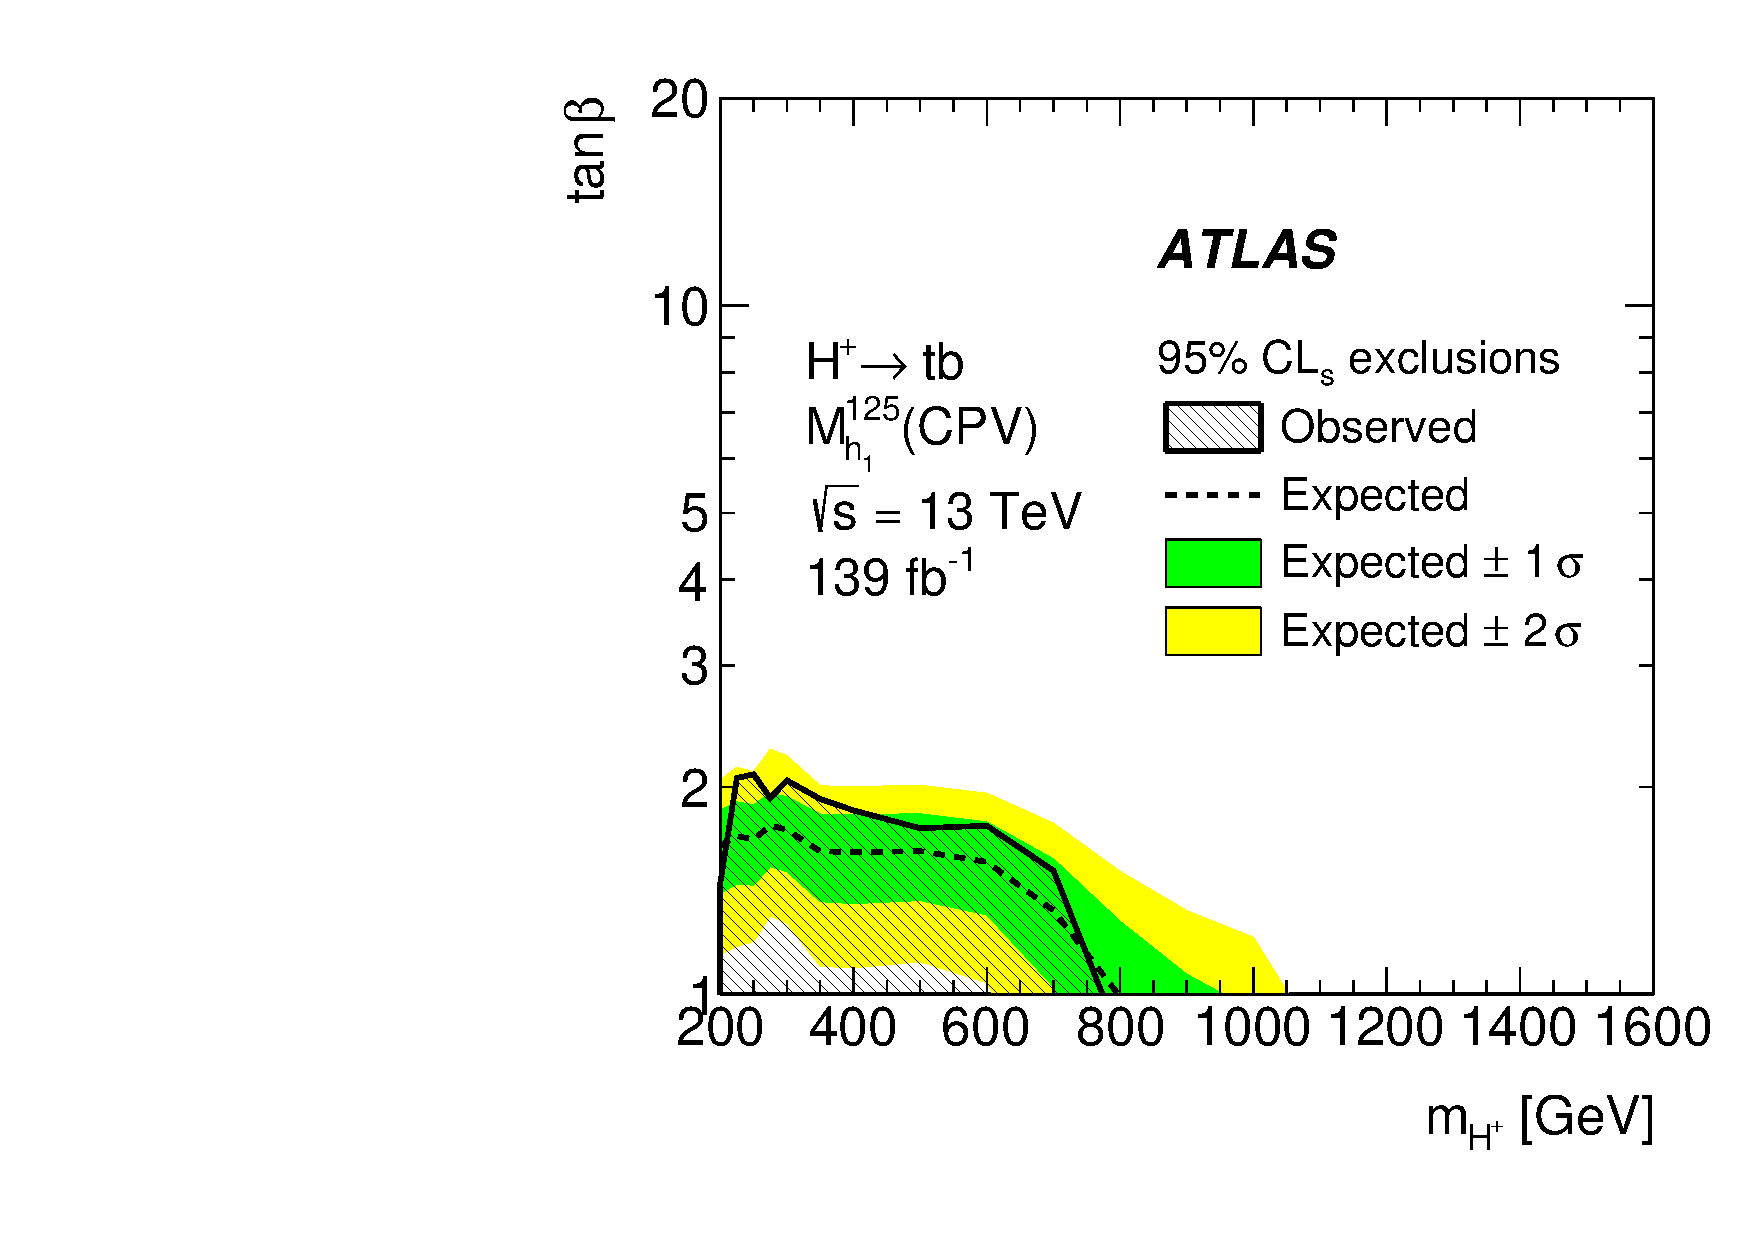
\includegraphics[width = 0.45\textwidth]{HPLUSTB/Fits/Exclusionplot_4FSS_mh1125_CPV_tb.pdf}} \\
    \caption{Observed and expected limits on $\tan\beta$ as a function of the $H^+$ mass in various scenarios: 
    (a) hMSSM, (b) $M_h^{125}$, (c) $M_h^{125}(\tilde{\chi})$, (d) $M_h^{125}(\tilde\tau)$, (e) $M_h^{125}$(alignment) and (f) $M_{h_1}^{125}$(CPV). 
    Limits are shown for $\tan\beta$ values in the range of 0.5--60 or 1--20 depending on the availability of model predictions. The bands surrounding the expected limits show the 68\% and 95\% confidence intervals.
    Uncertainties in the predicted $H^+$ cross-sections or branching ratios are not considered.}
    \label{Hplustb:exclusionstanb}
\end{figure}

\section{2HDM+a interpretation}

The $H^+$ upper limits results can also be interpreted in the context of the 2HDM+a model, as the production and decay modes, cross-sections and branching ratios of the charged Higgs bosons are identical in both models. The interpretation of $H^\pm\to tb$ results in this model is performed for the first time in the literature.\\

The 2HDM+a model~\cite{Bauer_2017,10.48550/arxiv.1810.09420} is built upon simplified Dark Matter~(DM) models, postulating a DM sector composed of a single fermionic DM particle and a pseudo-scalar mediator on top of the 2HDM assumption of building the Higgs sector with two complex Higgs doublets. In this particular model, the interactions between the \acrshort{SMlabel} and DM sectors are mediated by a pseudo-scalar $a$, although other models contemplate axial-vectors or scalars~\cite{Abercrombie_2020,10.48550/arxiv.1603.04156,10.48550/arxiv.1703.05703}. The choice of type of particle is motivated by the potential sensitivity in collider searches, as direct-detection of pseudo-scalars is suppressed~\cite{Abe_2019} and a dedicated search will not provide strong constraints.\\

The phenomenology of the model has the five Higgs bosons from the 2HDM sector: a light CP even boson $h$, a heavy CP-even boson $H$, a CP-odd boson $A$ and the charged bosons $H^+$. As in the previous models, the Type-II structure is considered together with the alignment limit~\cite{Gunion_2003}, to identify the $h$ state with the \acrshort{SMlabel} Higgs boson. The mediator $a$ couples the \acrshort{SMlabel} fermions with the Dirac DM particle $\chi$. In addition, $a$ couples to \acrshort{SMlabel} fermions proportionally to the Yukawa couplings and mixes with $A$ with a mixing angle $\theta$. Figure~\ref{Hplustb:2hdmafeynman} shows a Feynman diagram with an interaction involving the $H^+$, $a$ and $\chi$ particles. A total of 14 parameters are needed to fully determine the model: the masses of the five 2HDM Higgs bosons; the mass of the mediator $a$; the mass of the DM $\chi$; the coupling between $a$ and $\chi$, $g_\chi$; the \acrshort{EW} \acrshort{VEV}, $v$; the \acrshort{VEV}s 2HDM ratio, $\tan\beta$; the mixing angles of the CP-even and CP-odd states, $\alpha$ and $\theta$, respectively; and three quartic couplings between the scalar doublets and the mediator.\\

\begin{figure}[htb]
    \RawFloats
    \centering
    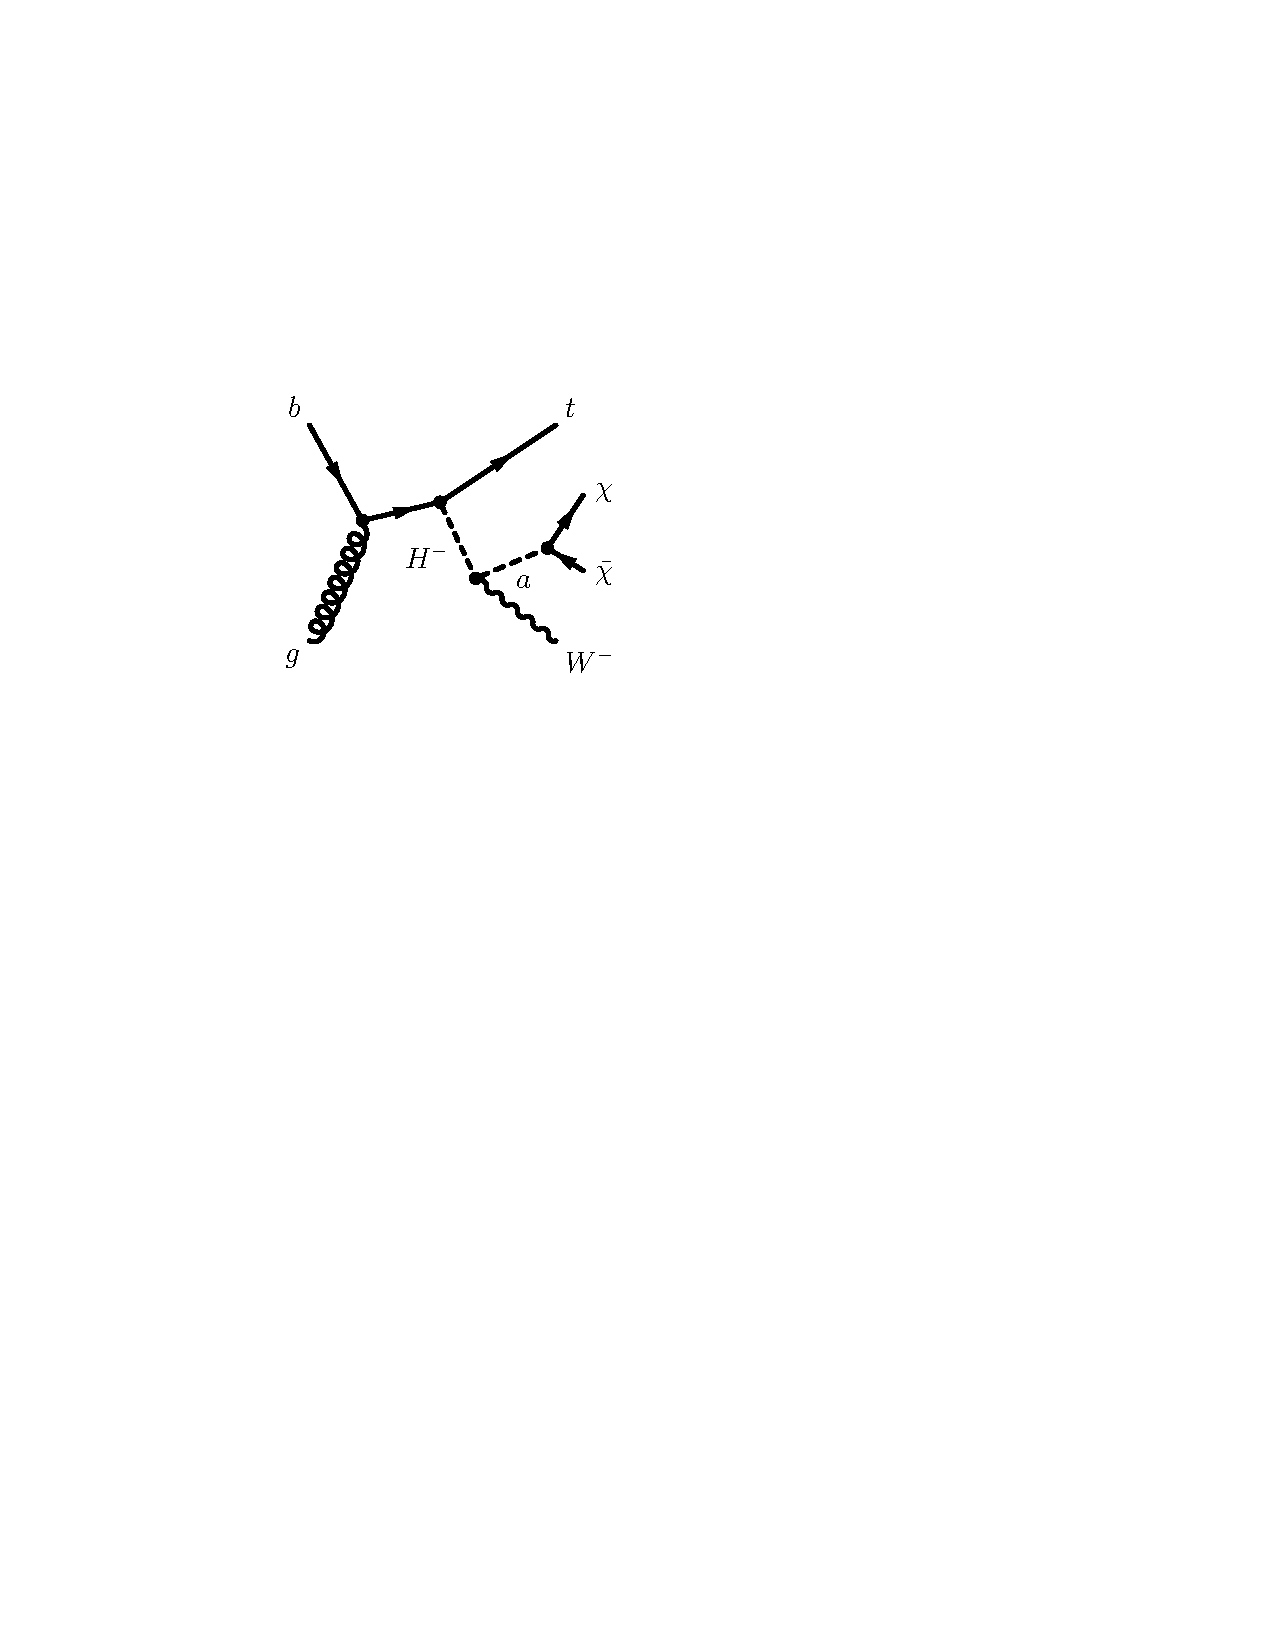
\includegraphics[width = 0.45\textwidth]{HPLUSTB/DM/feynmanHmin.pdf}
    \caption{Representative Feynman diagram for the dominant gluon-induced production and decay mode in the 2HDM+a involving a charged Higgs boson, the DM particle, $\chi$ and the pseudo-scalar mediator, $a$.}
    \label{Hplustb:2hdmafeynman}
\end{figure}

This model predicts a wide variety of signatures and \acrshort{ATLASlabel} has summary results that consist in various dark matter searches using 139~fb$^{-1}$ data~\cite{Hpluscomb}. The most prominent signatures, the production of DM in association with a Higgs boson $\MET+h(\bbar)$~\cite{2108.13391} and with a $Z$ boson $\MET+Z(\ell^+\ell^-)$ are used in a combined likelihood fit for the statistical combination. Further signatures are related to DM production in association with a top quark and a W boson (\MET+$Wt$), visible decays of the additional heavy Higgs bosons, and invisible decays of the SM Higgs boson to DM.\\

The nominal $H^+$ samples are compared to samples generated with different 4FS 2HDM+a models for a range of relevant kinematic variables to verify that the signal signatures are the same, and hence the interpretation is possible. Figure~\ref{Hplustb:2hdmatruth} shows the similarity of the truth jet multiplicity distributions corresponding to for various models in two $H^+$ example masses.\\

\begin{figure}[htb]
    \RawFloats
    \centering
    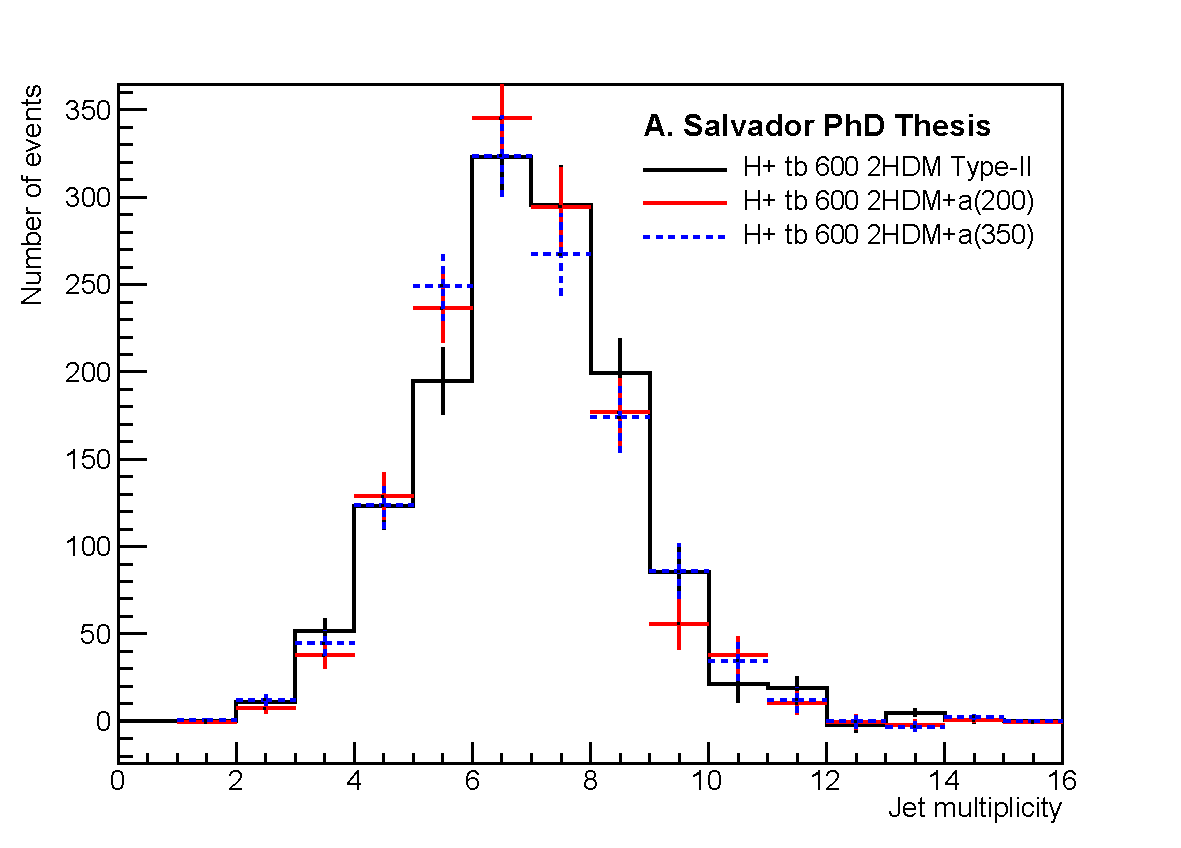
\includegraphics[width = 0.49\textwidth]{HPLUSTB/DM/njets_600.pdf}
    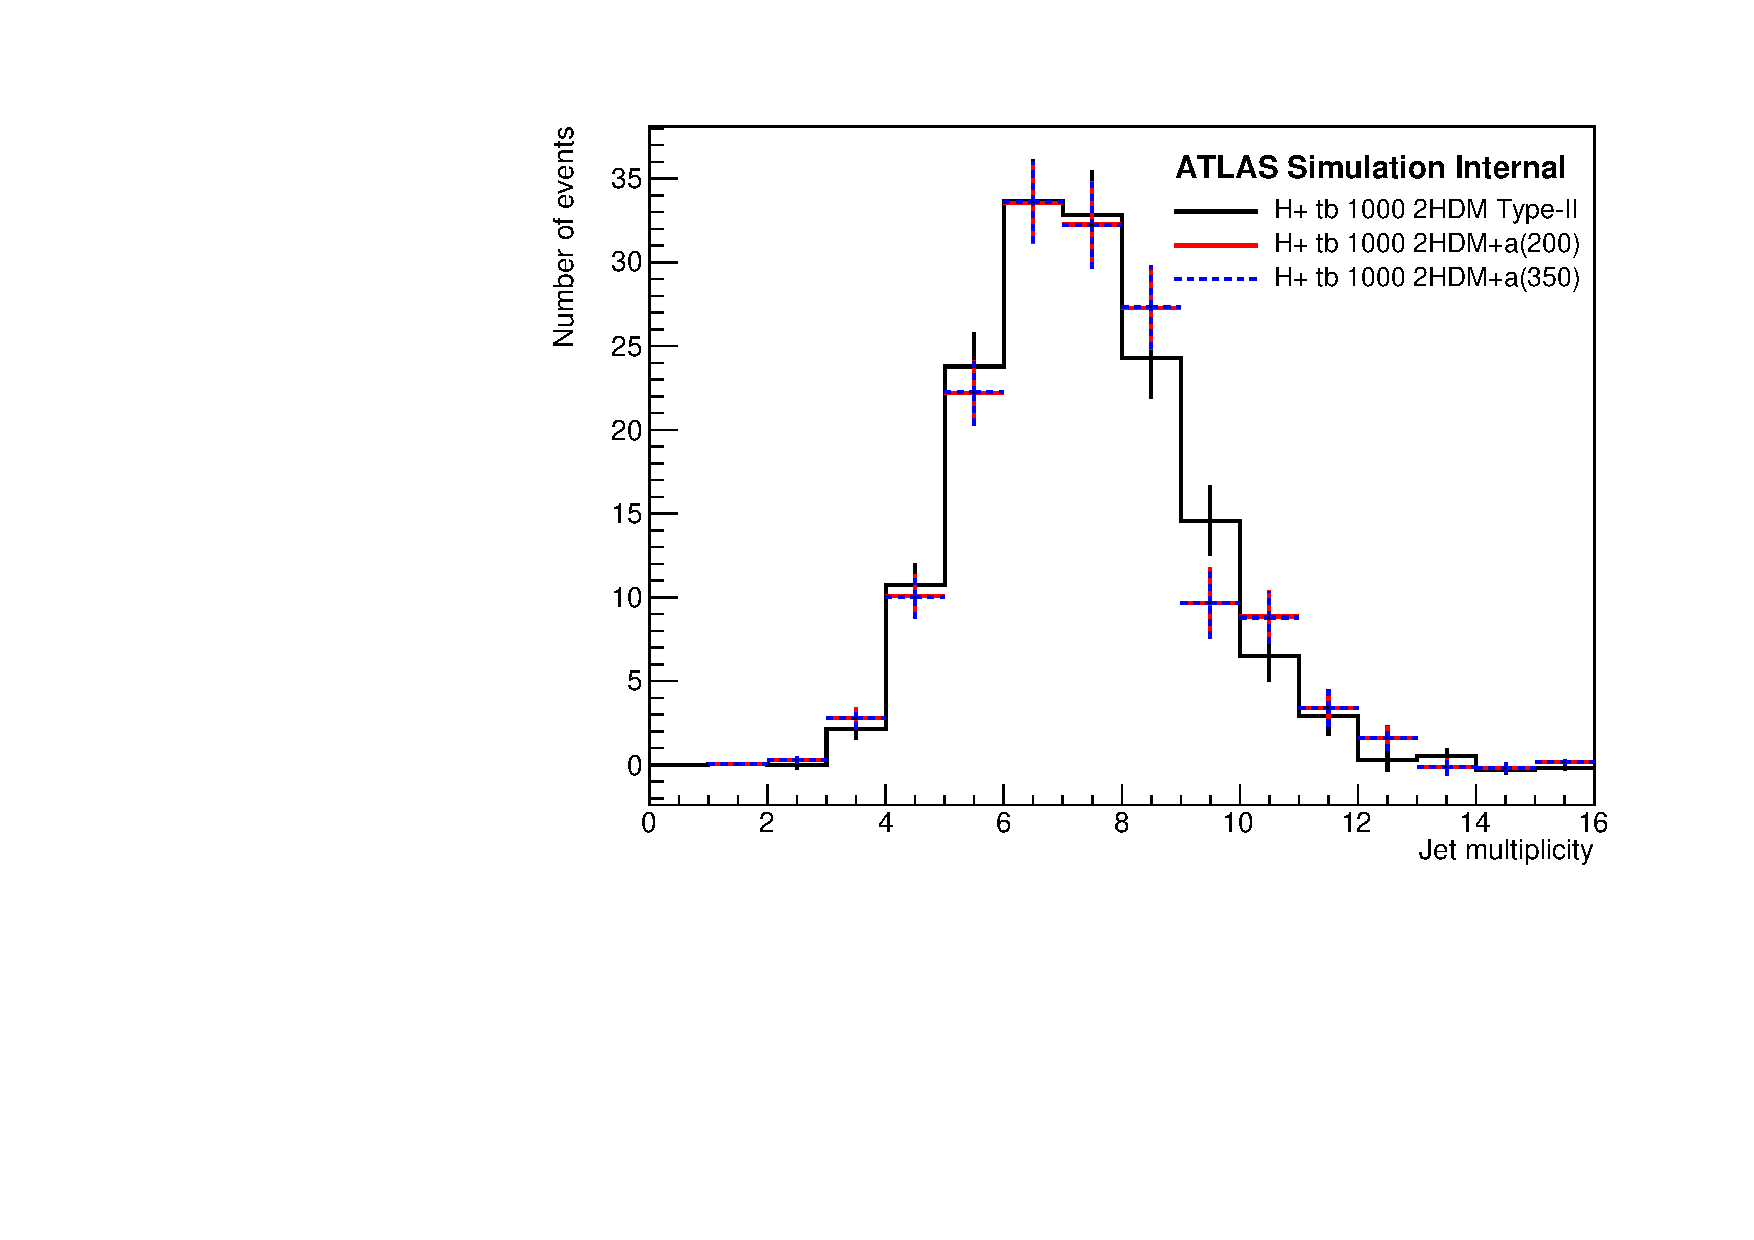
\includegraphics[width = 0.49\textwidth]{HPLUSTB/DM/njets_1000.pdf}
    \caption{Multiplicity of truth jets with $\pT>25$~GeV corresponding to the 600 GeV (left) and 1000 GeV (right) $H^+$ samples. The black line corresponds to the 4FS 2HDM Type-II NLO model while the red and blue lines correspond to the 4FS 2HDM+a NLO generated with $a$ masses of 200 and 350 GeV.}
    \label{Hplustb:2hdmatruth}
\end{figure}

To generate the exclusion figures, predictions for the $pp\to tbH^+$ cross-section and B($H^+\to tb$) have been computed for the 4FS 2HDM+a NLO model for different values: $\sin\theta\in[0.1,0.9]$, $\tan\beta\in[0.3,50]$, $m_a\in[100\text{ GeV},800\text{ GeV}]$, $m_{H^+}\in[200\text{ GeV},1000\text{ GeV}]$ and $m_\chi\in[20\text{ GeV},500\text{ GeV}]$.\\

Figure~\ref{Hplustb:BRprodexclmassvsmass} shows the dependence of B($H^+\to tb$) and the production of the signal as a function of $m_{H^+}$ and $m_a$, for $\sin\theta=0.35,0.7$ and $\tan\beta=1$. As expected, the branching fraction depends on both masses and is $\sim$100\% until $m_{H^+} > m_a+80$~GeV, when the $H^+\to aW$ and $H^+\to WH$ decays are allowed. The corresponding cross-section does not change with $\sin\theta$.\\

Figure~\ref{Hplustb:exclvsmass} shows the exclusion contour extracted in the $m_{H^+}$--$m_a$ plane from the analysis limits and the predicted production in the 2HDM+a. The dependence of the contour on $m_a$ is not substantial since the sensitivity of the $H^+$ analysis is not directly focused on the properties of $a$.\\

\begin{figure}[htb]
    \RawFloats
    \centering
       \subfloat[]
       {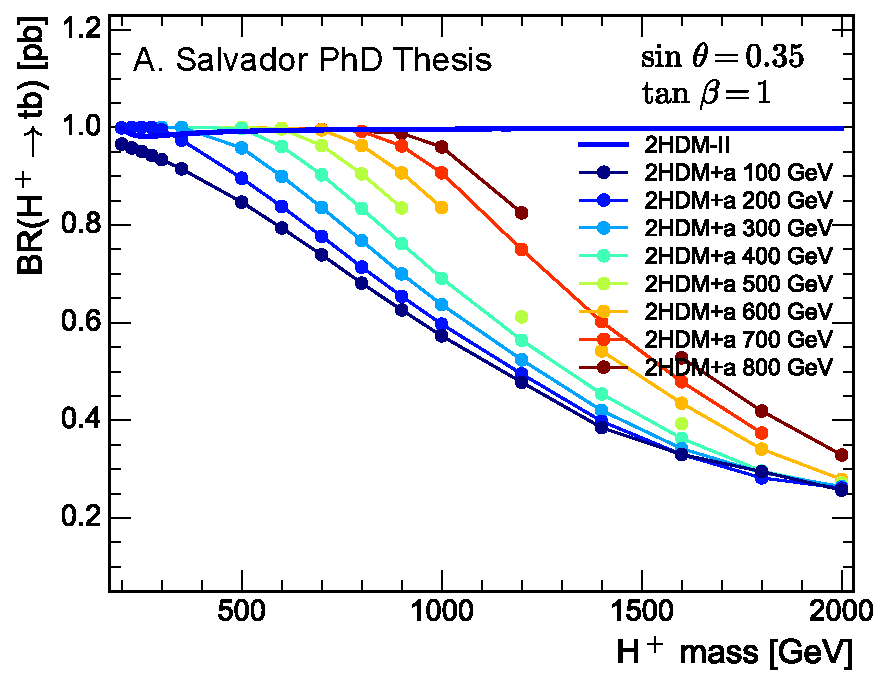
\includegraphics[width = 0.49\textwidth]{HPLUSTB/DM/BR2HDMa035.pdf}} 
       \subfloat[]
       {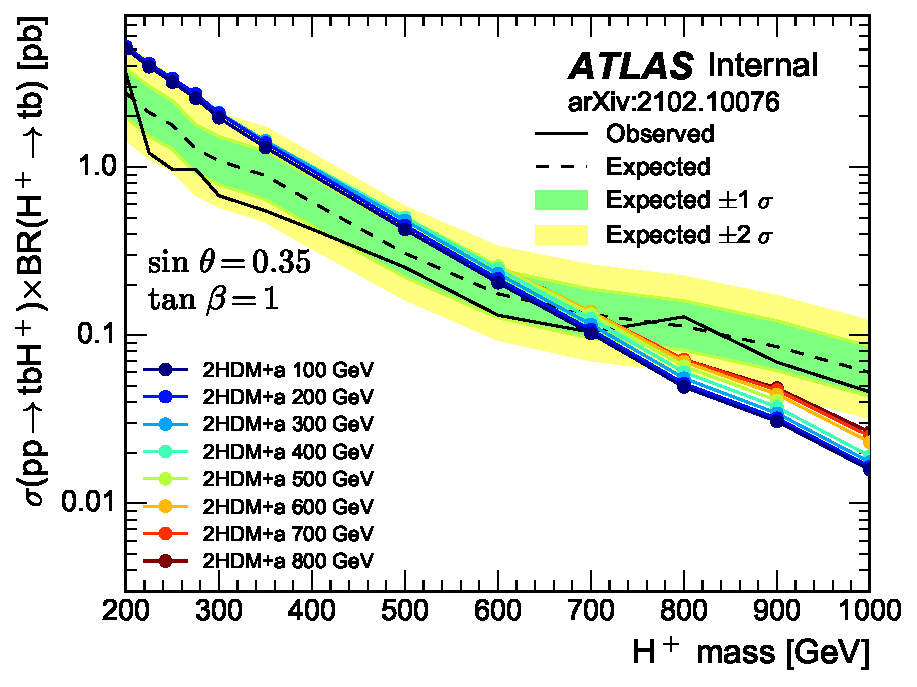
\includegraphics[width = 0.49\textwidth]{HPLUSTB/DM/Limit2HDMa035.pdf}} \\
       {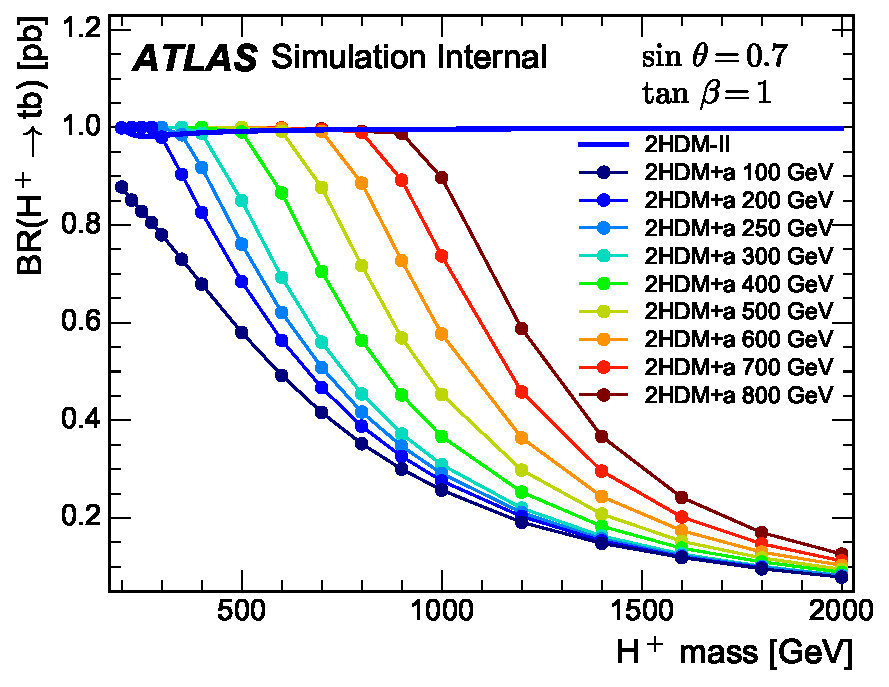
\includegraphics[width = 0.49\textwidth]{HPLUSTB/DM/BR2HDMa07.pdf}} 
       \subfloat[]
       {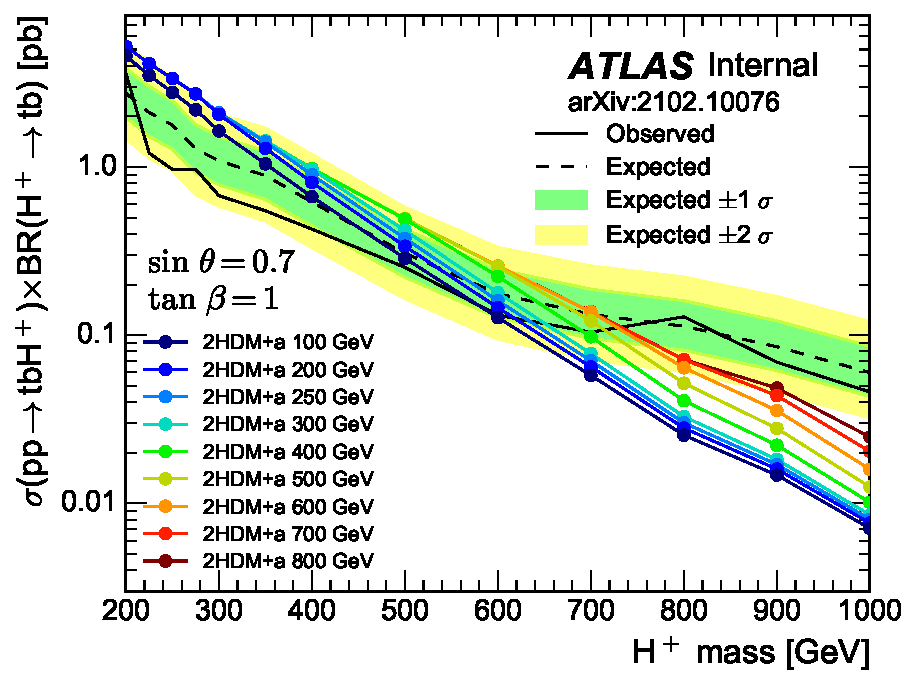
\includegraphics[width = 0.49\textwidth]{HPLUSTB/DM/Limit2HDMa07.pdf}} 
    \caption{(a) and (c) Branching ratio of $H^+\to tb$ as a function of the $H^+$ mass for $\sin\theta=0.35(0.7)$ at the top(bottom). Predictions are compared between the 2HDM Type-II (2HDM-II) and 2HDM+a for various $a$ masses. (b) and (d) Expected and observed cross-section times branching ratio limits of the $H^+$ process, with various 2HDM+a predictions overlaid.}
    \label{Hplustb:BRprodexclmassvsmass}
\end{figure}

\begin{figure}[htb]
    \RawFloats
    \centering
       {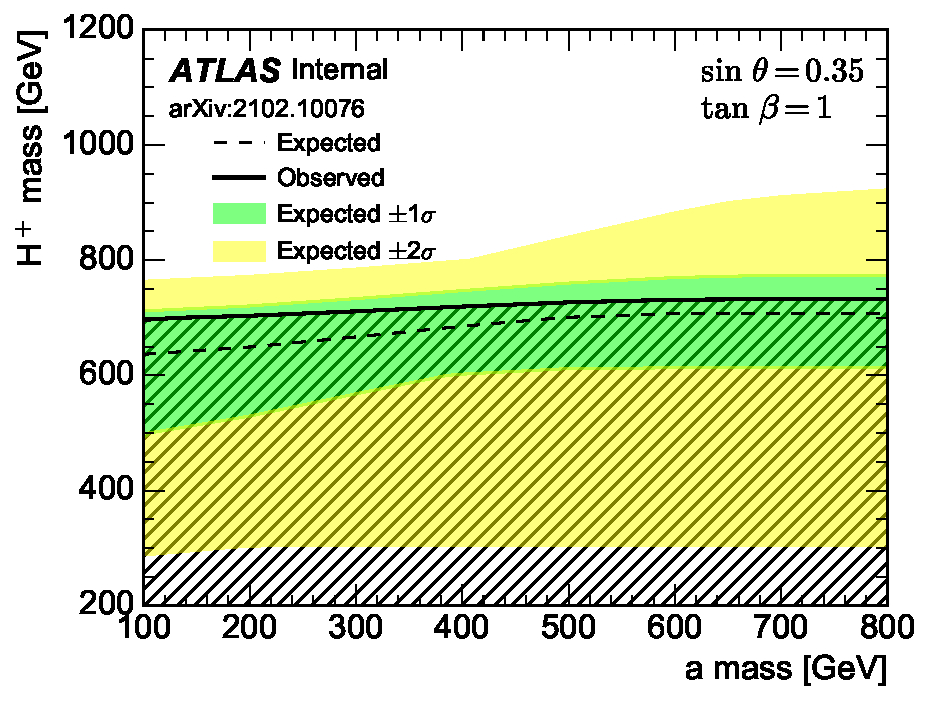
\includegraphics[width = 0.6\textwidth]{HPLUSTB/DM/2HDMa035.pdf}} \\
       {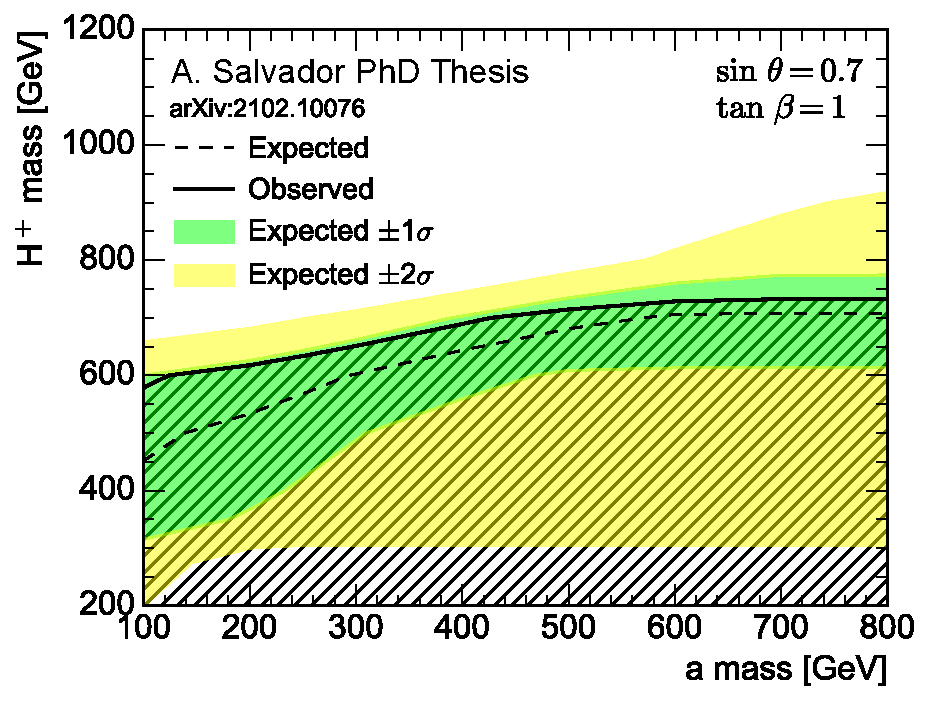
\includegraphics[width = 0.6\textwidth]{HPLUSTB/DM/2HDMa07.pdf}} 
    \caption{Observed and expected exclusion plots in the $H^+$--$a$ mass plane of the production of $H^+\to tb$ for $\sin\theta=0.35$ (0.7) at the top (bottom).}
    \label{Hplustb:exclvsmass}
\end{figure}

Figure~\ref{Hplustb:2HDMa_mA_ma} shows the exclusion contours including other \acrshort{ATLASlabel} DM searches. The $\MET+ Z(\ell^+\ell^-)$ and $\MET+ h(\bbar)$ searches dominate the sensitivity across the two parameter planes, expected from the resonant production of the pseudo-scalars. The $H^+$ results provide complementary sensitivity to the $\MET+ X$ searches. The corresponding exclusion contour shows only a moderate dependence on $m_a$.\\

\begin{figure}[htb]
    \RawFloats
    \centering
    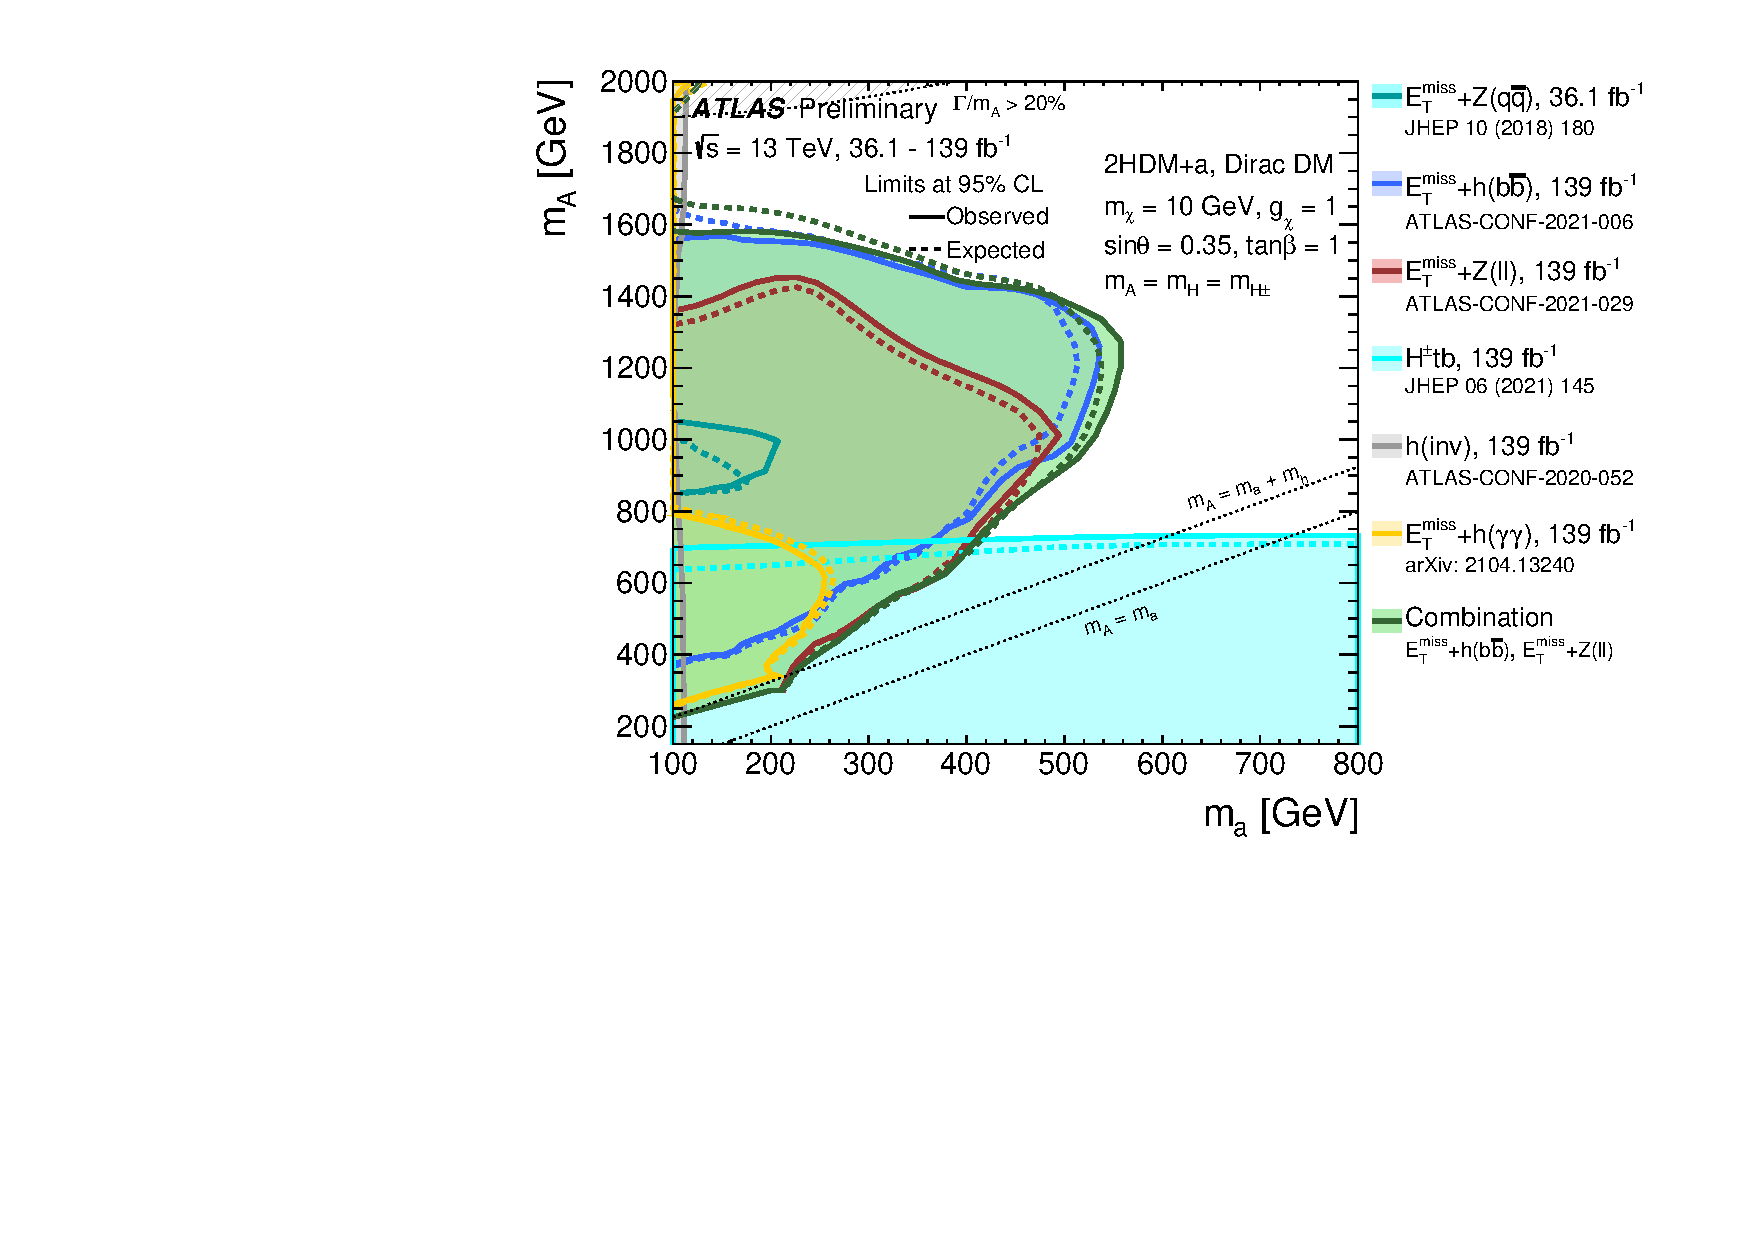
\includegraphics[width = 0.495\textwidth]{HPLUSTB/DM/mA_ma_035_1_10.pdf}
    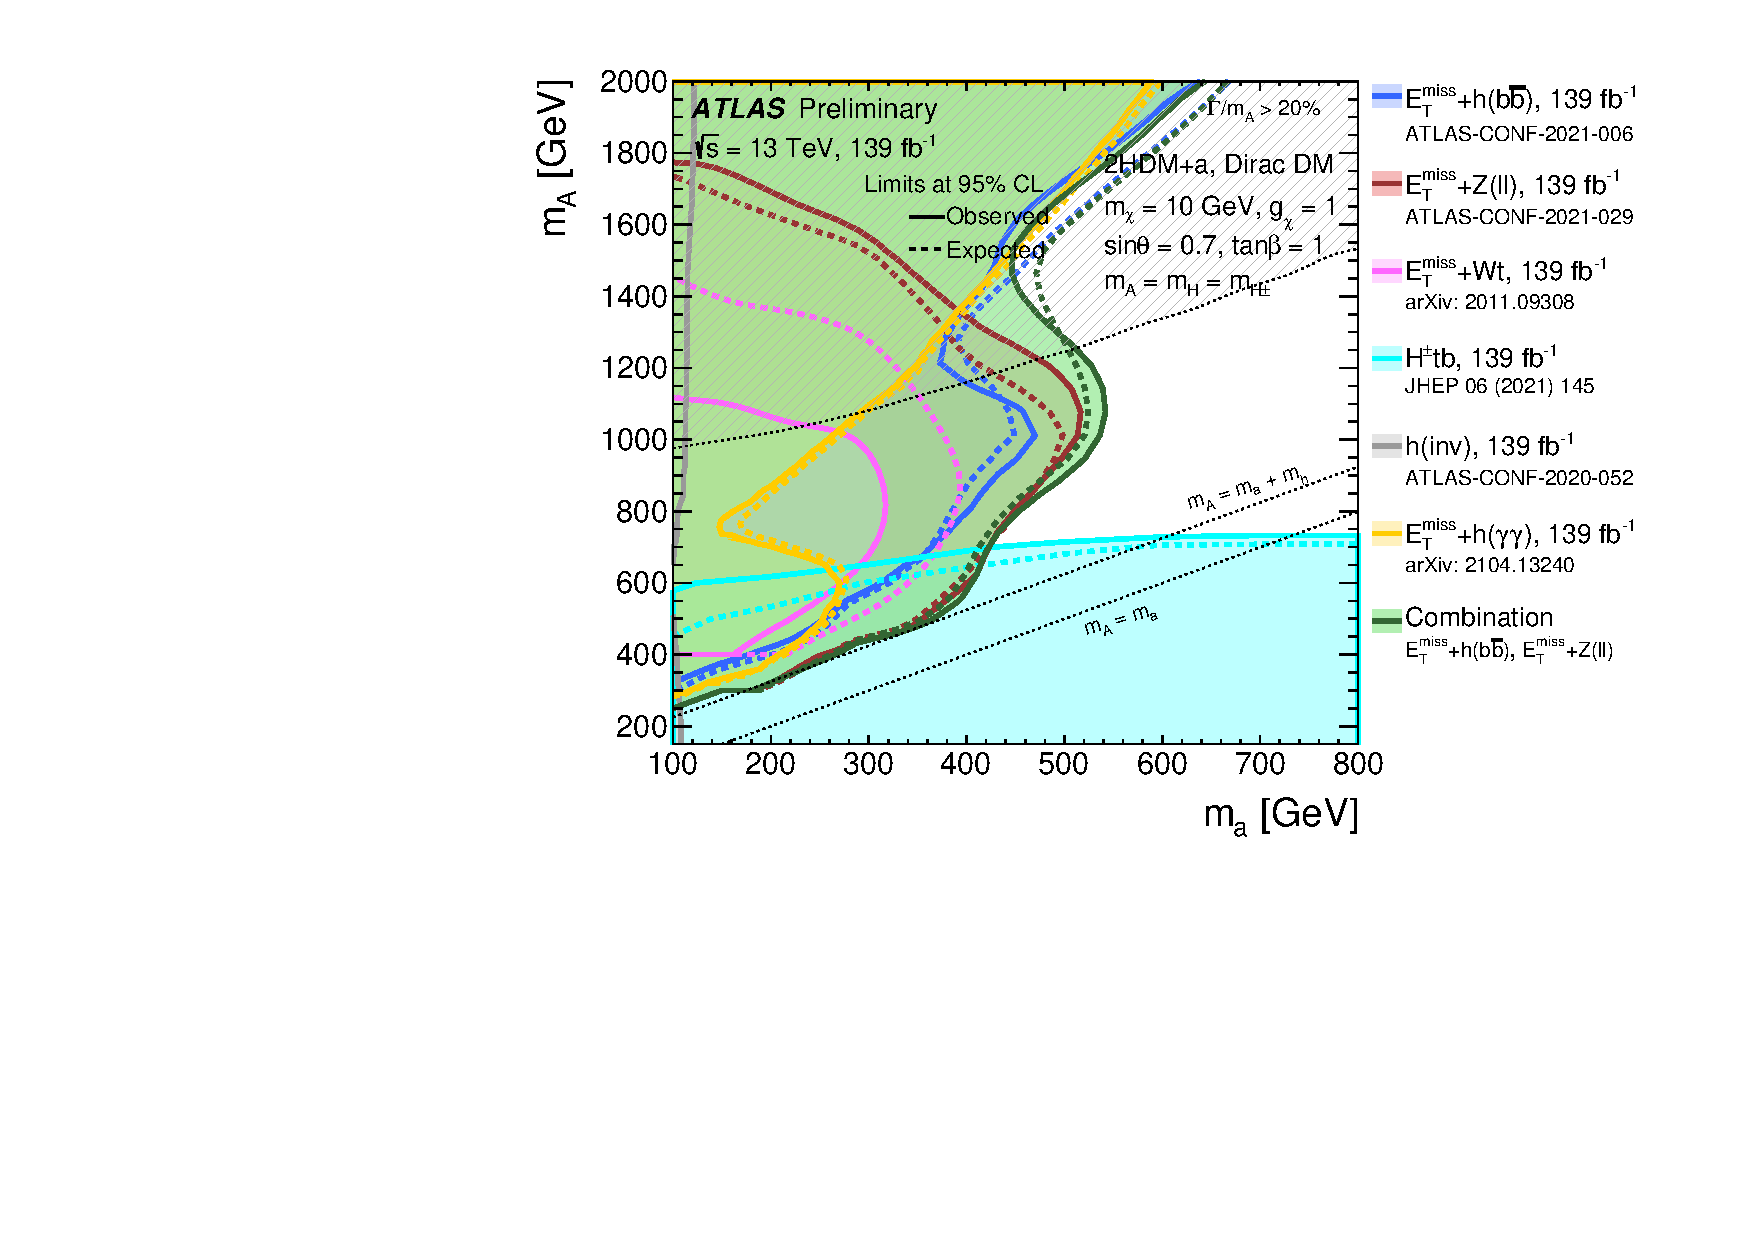
\includegraphics[width = 0.495\textwidth]{HPLUSTB/DM/mA_ma_07_1_10.pdf}
    \caption{Observed (solid lines) and expected (dashed lines) exclusion regions at 95\% CL in the $m_a$--$m_A$ plane with $\sin\theta=0.35$ (left) and $\sin\theta=0.7$ (right). The results are shown for several individual searches as well as the combination of the $\MET+Z(\ell^+\ell^-)$ and $\MET+h(\bbar)$ searches. The dashed grey regions indicate the region where the width of the Higgs bosons exceeds 20\% of its mass.}
    \label{Hplustb:2HDMa_mA_ma}
\end{figure}

Figure~\ref{Hplustb:2HDMa_tanb_mA} shows the exclusion contours as a function of $m_A$ and $\tan\beta$, for $\sin\theta=0.35,0.7$ and $m_a=250$~GeV. Similarly, the parameter space is almost fully excluded by the $\MET+ Z(\ell^+\ell^-)$ search, except that the $\MET+ Wt$ search also excludes the low $\tan\beta$ region for large values of $m_A$. In addition, the $H^+\to tb$ search provides complementary sensitivity to the other searches, although with a moderate dependence in the lower parameter region.\\

\begin{figure}[htb]
    \RawFloats
    \centering
    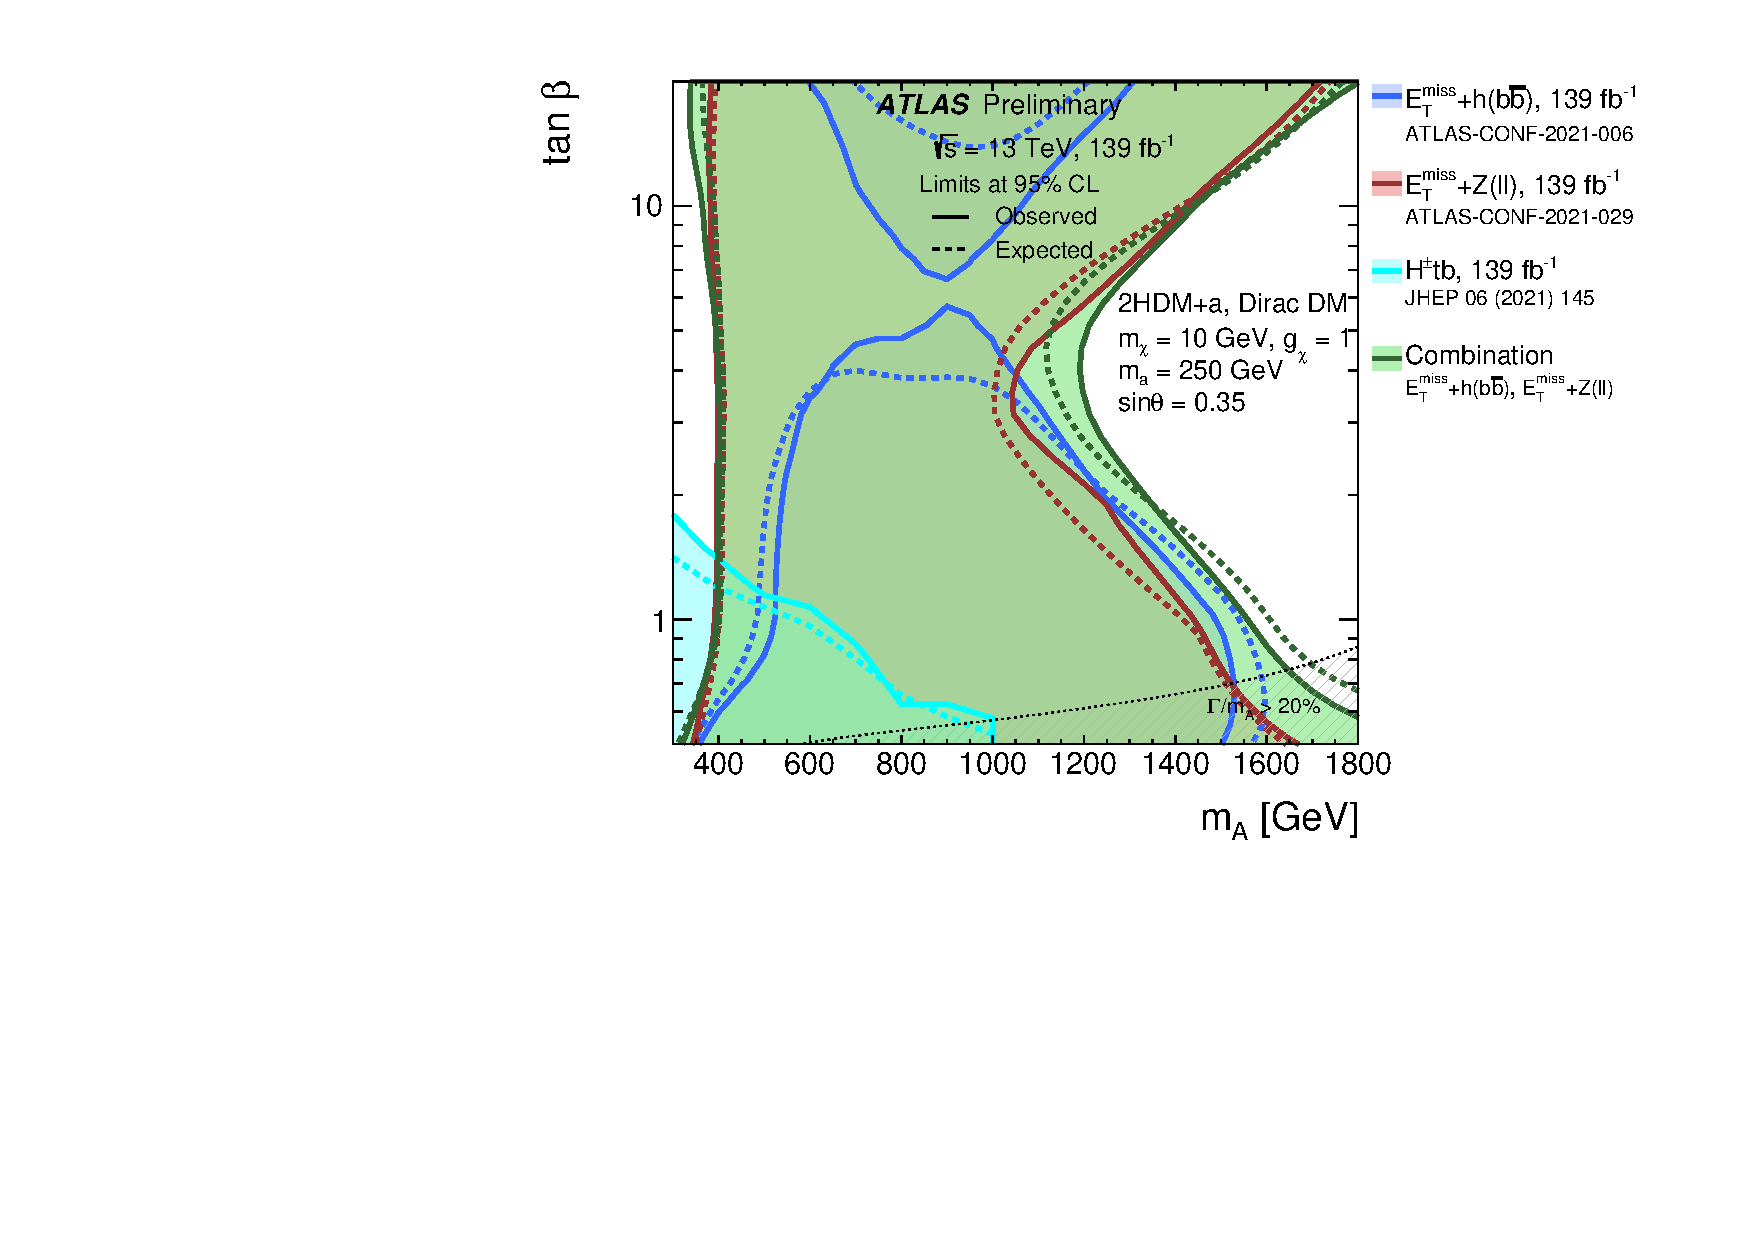
\includegraphics[width = 0.495\textwidth]{HPLUSTB/DM/tanb_mA_035_250_10.pdf}
    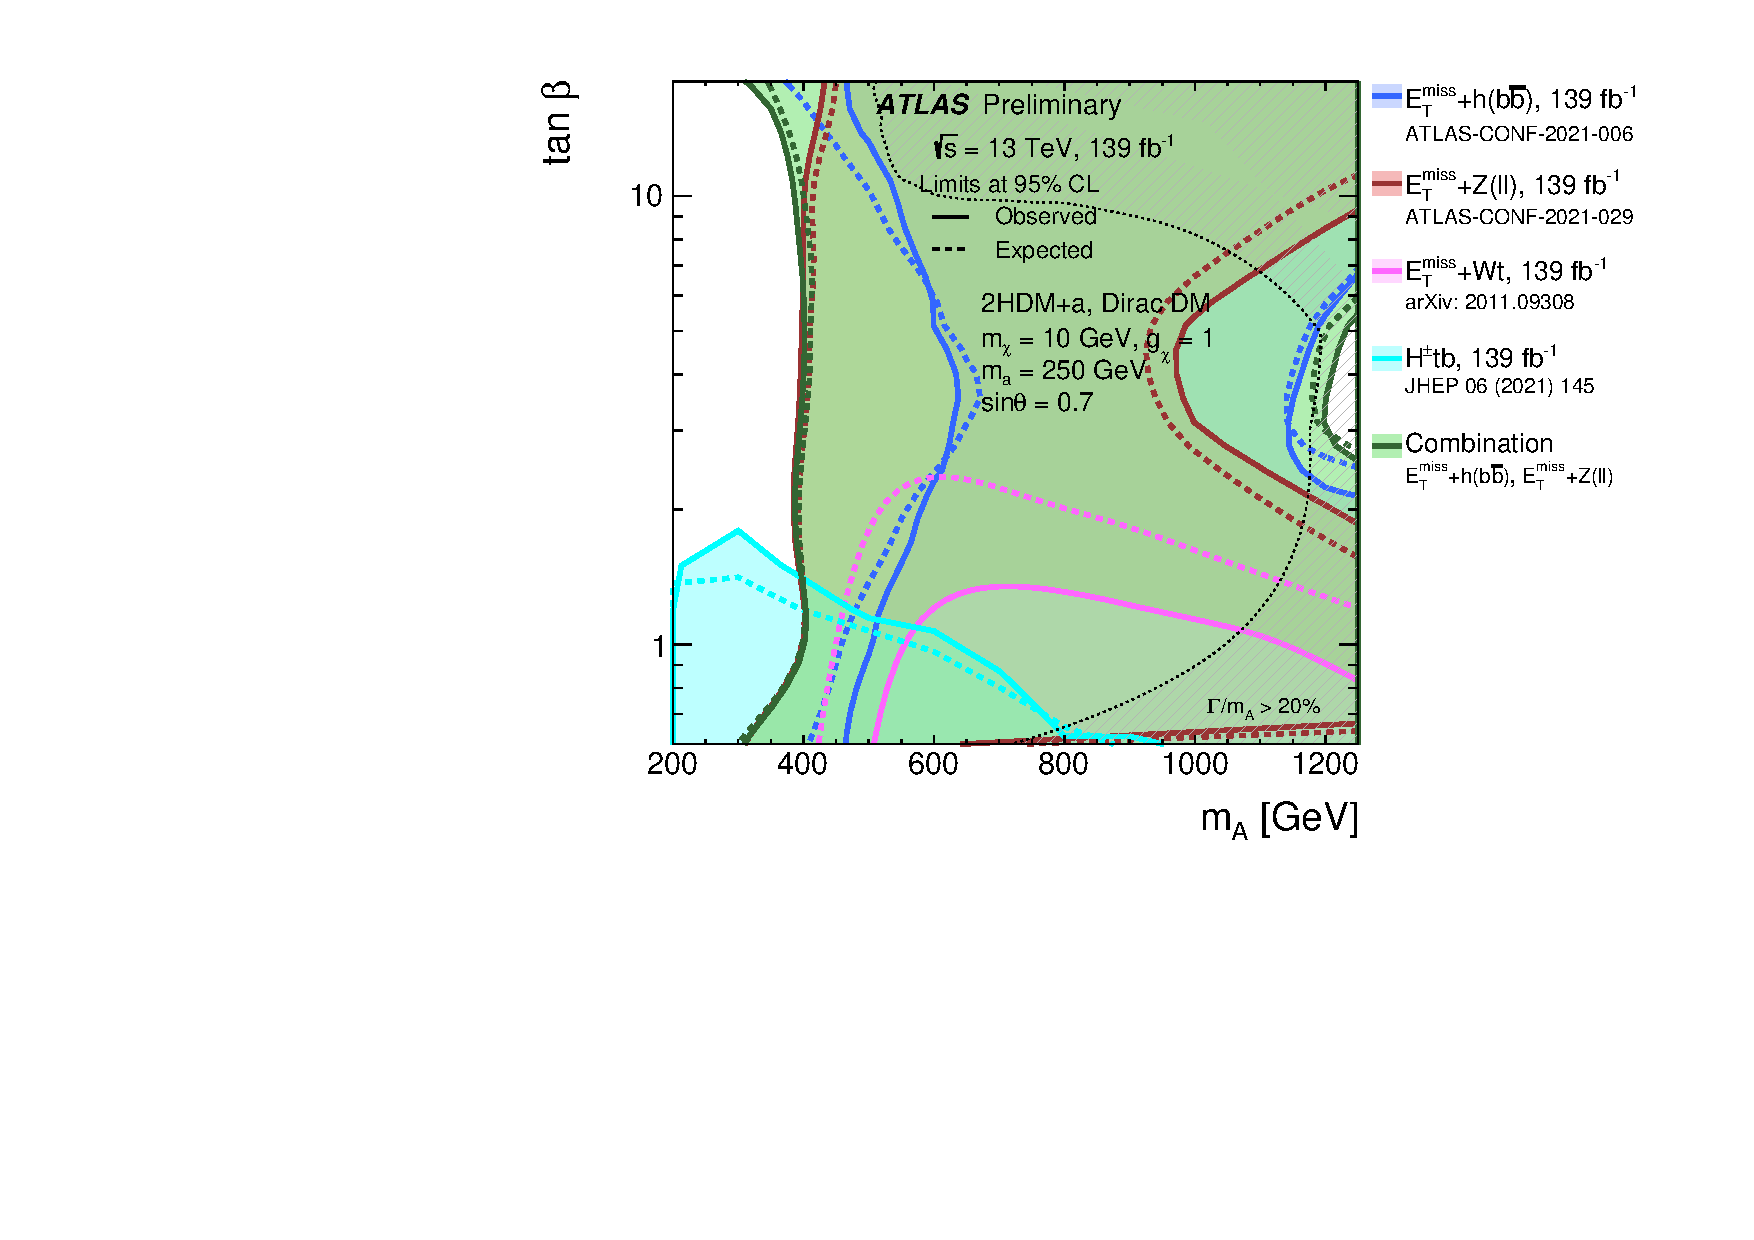
\includegraphics[width = 0.495\textwidth]{HPLUSTB/DM/tanb_mA_07_250_10.pdf}
    \caption{Observed (solid lines) and expected (dashed lines) exclusion regions at 95\% CL in the $m_A$--$\tan\beta$ plane with $\sin\theta=0.35$ (left) and $\sin\theta=0.7$ (right). The results are shown for several individual searches as well as the combination of the $\MET+Z(\ell^+\ell^-)$ and $\MET+h(\bbar)$ searches. The dashed grey regions indicate the region where the width of the Higgs bosons exceeds 20\% of its mass.}
    \label{Hplustb:2HDMa_tanb_mA}
\end{figure}

Figure~\ref{Hplustb:2HDMa_tanb_ma} shows a similar scan to the one inFigure~\ref{Hplustb:2HDMa_tanb_mA} but varying the $m_a$ and setting $m_A=600$~GeV. Again, the strongest exclusion is observed from the $\MET+ Z(\ell^+\ell^-)$ and $\MET+ h(\bbar)$ searches. An increase in the exclusion range is found for large values of $\tan\beta$, related to the contributions from $\bbar$-initiated signal production, dominant at large values of $\tan\beta$. The $H^+\to tb$ search provides complementary sensitivity at low $\tan\beta$ values with very small dependence on $m_a$.\\

\begin{figure}[htb]
    \RawFloats
    \centering
    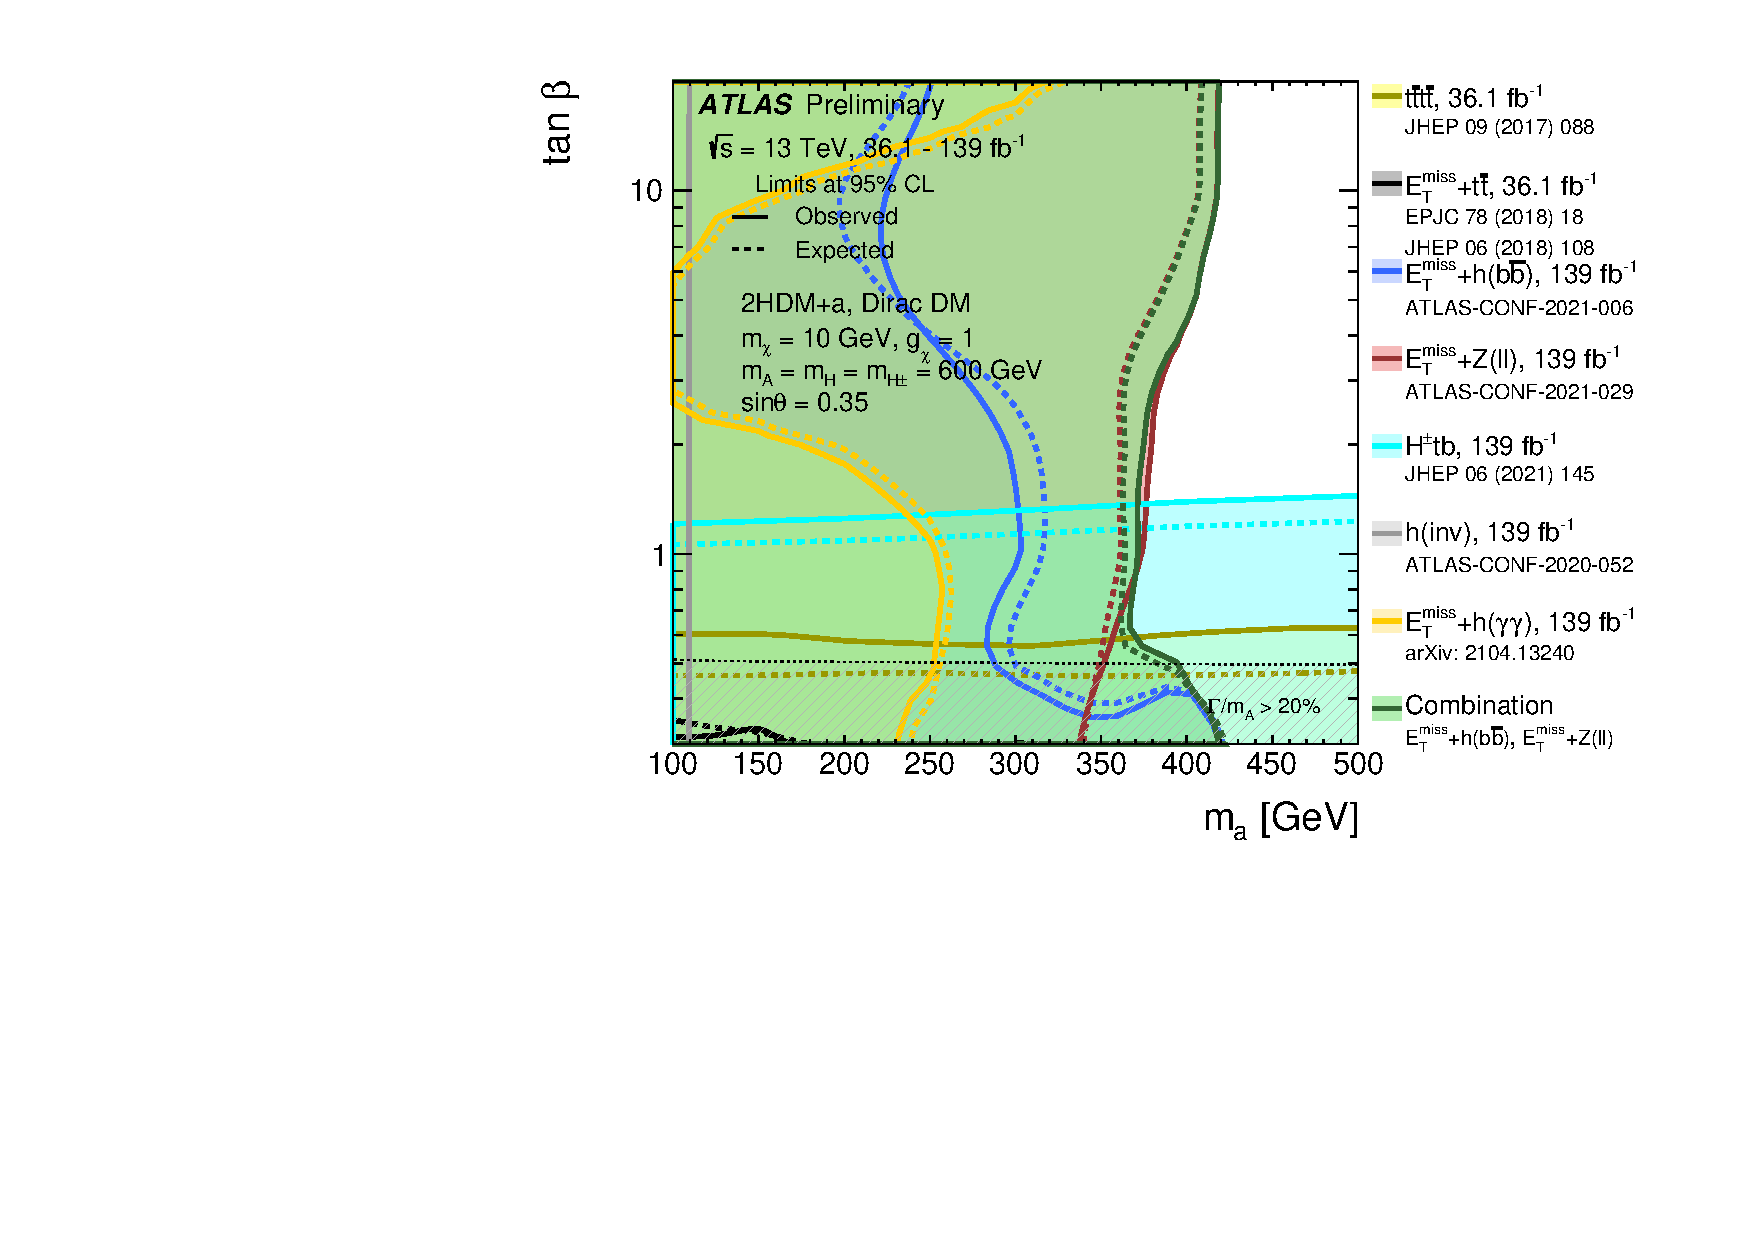
\includegraphics[width = 0.495\textwidth]{HPLUSTB/DM/tanb_ma_035_600_10.pdf}
    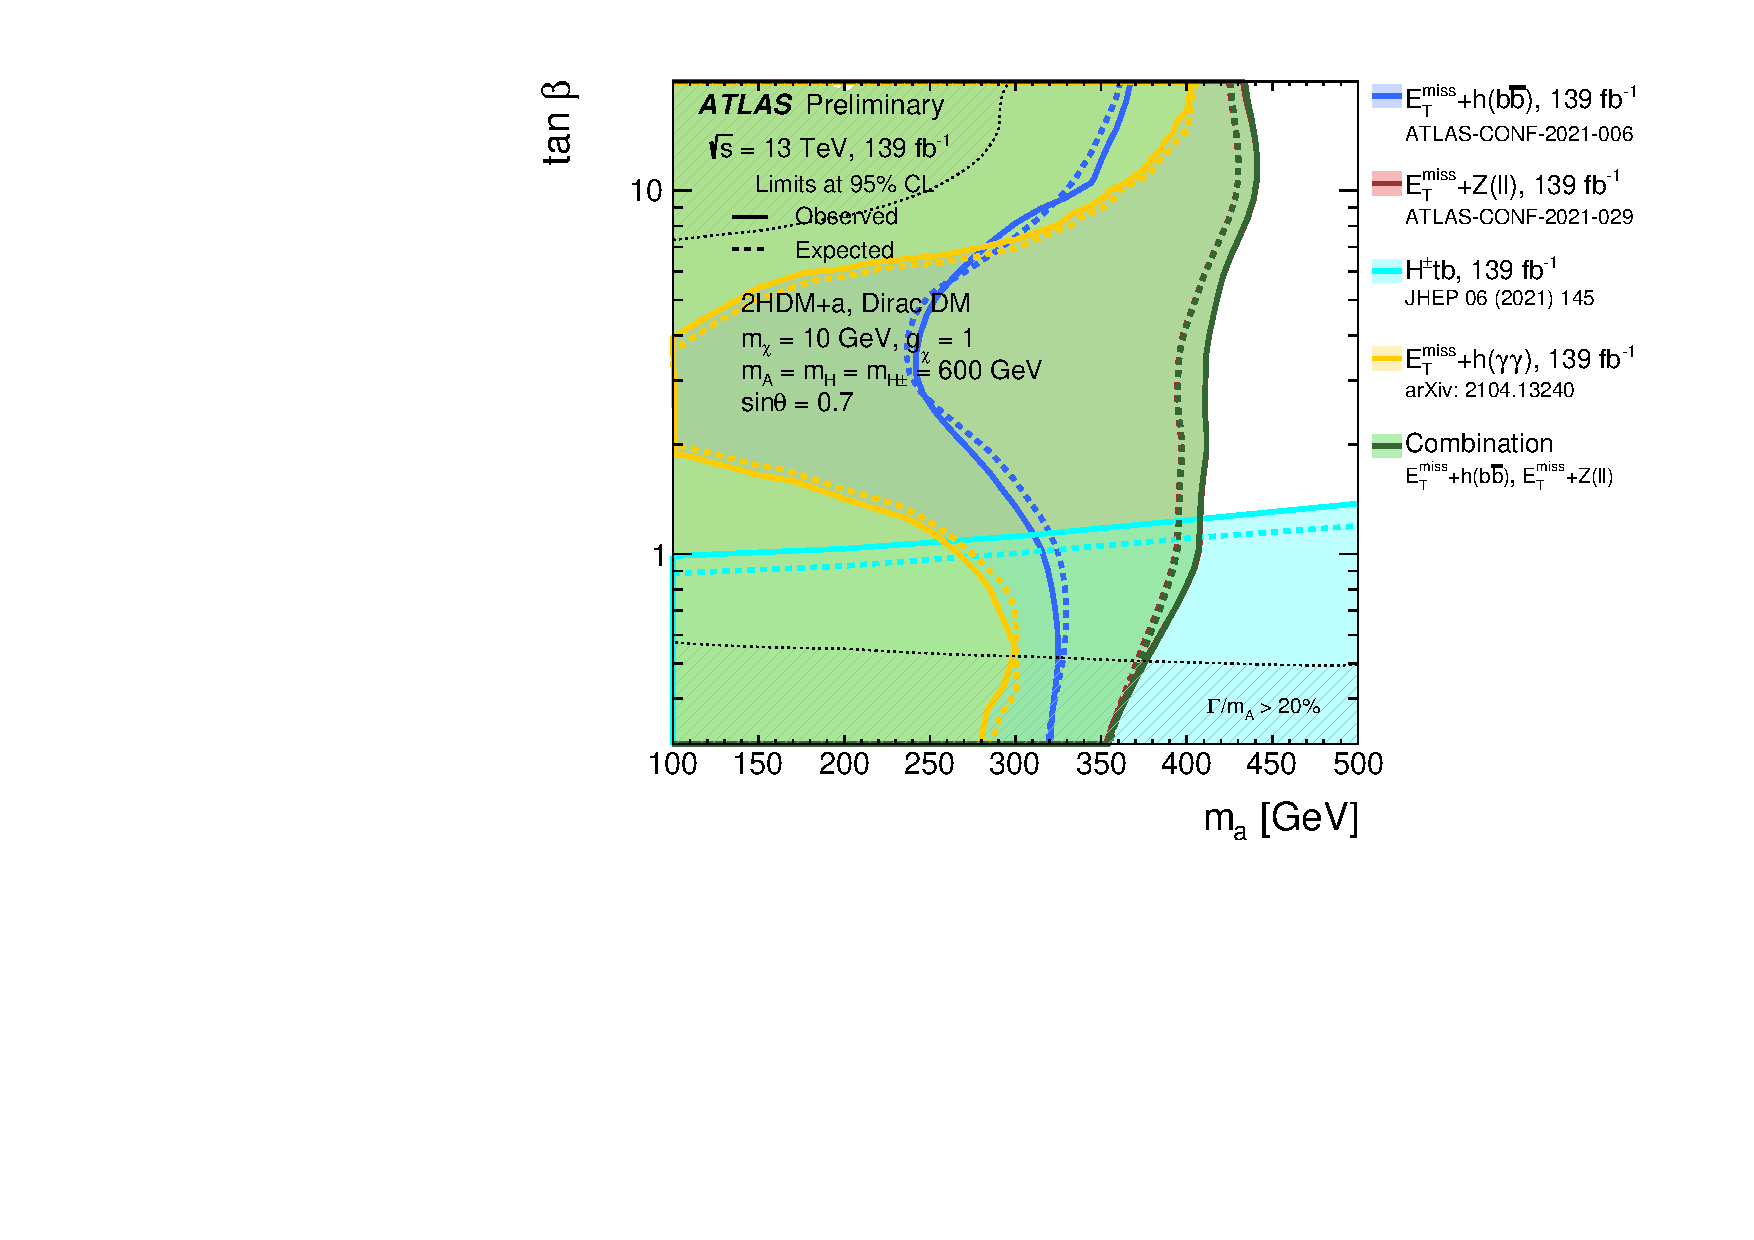
\includegraphics[width = 0.495\textwidth]{HPLUSTB/DM/tanb_ma_07_600_10.pdf}
    \caption{Observed (solid lines) and expected (dashed lines) exclusion regions at 95\% CL in the $m_a$--$\tan\beta$ plane with $\sin\theta=0.35$ (left) and $\sin\theta=0.7$ (right). The results are shown for several individual searches as well as the combination of the $\MET+Z(\ell^+\ell^-)$ and $\MET+h(\bbar)$ searches. The dashed grey regions indicate the region where the width of the Higgs bosons exceeds 20\% of its mass.}
    \label{Hplustb:2HDMa_tanb_ma}
\end{figure}

Figure~\ref{Hplustb:2HDMa_sintheta} shows the exclusion limits as a function of $\sin\theta$ for the 2HDM+a model for two pairs of masses $m_a,m_A = 200, 600$~GeV and $m_a,m_A=350,1000$~GeV. The strongest exclusion in the medium $\sin\theta$ range is provided by the $\MET+ Z(\ell^+\ell^-)$ and $\MET+ h(\bbar)$ searches. The $H^+\to tb$ signature shows a different $\sin\theta$ dependence compared to the other signatures as it is not directly sensitive to the neutral boson production. However, it is particularly sensitive at very small mixing angles.\\

\begin{figure}[htb]
    \RawFloats
    \centering
    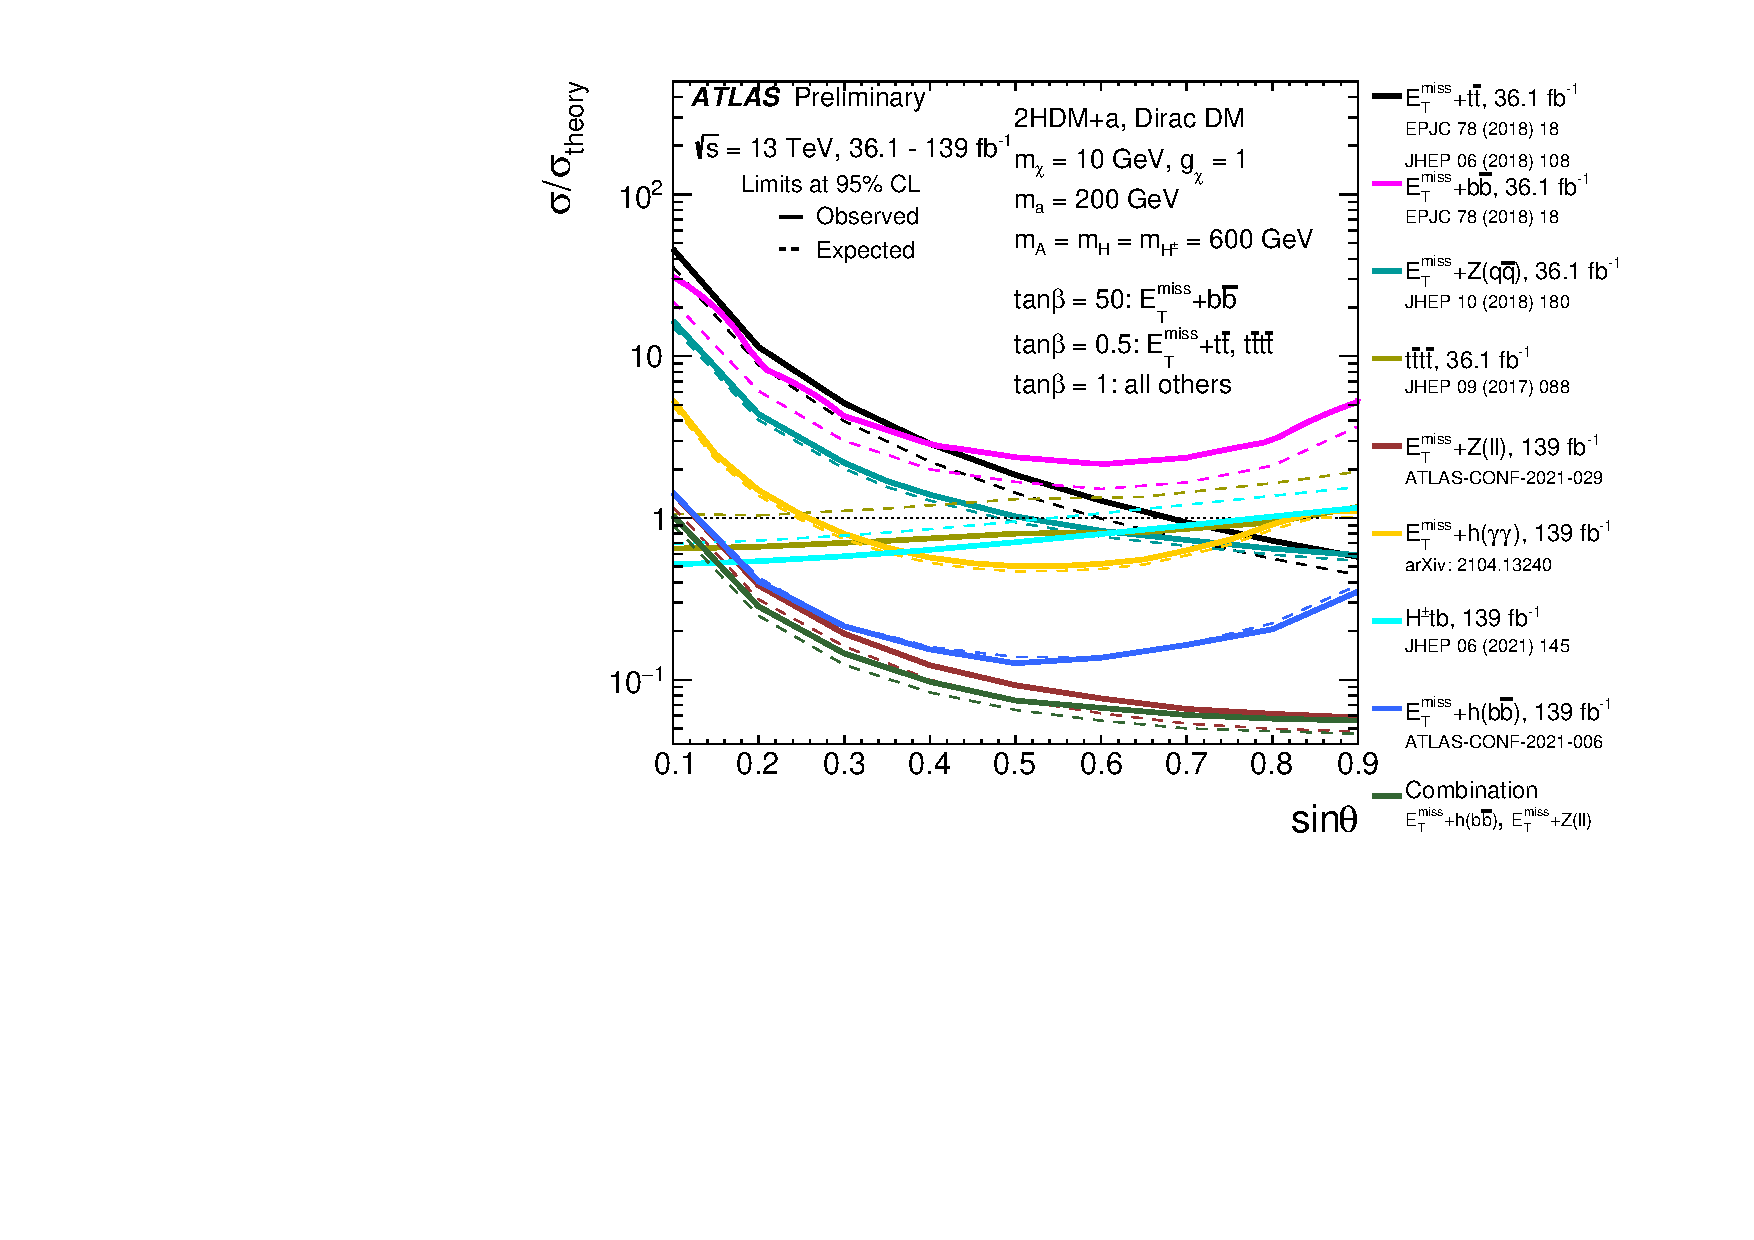
\includegraphics[width = 0.495\textwidth]{HPLUSTB/DM/sin_200_600_1_10.pdf}
    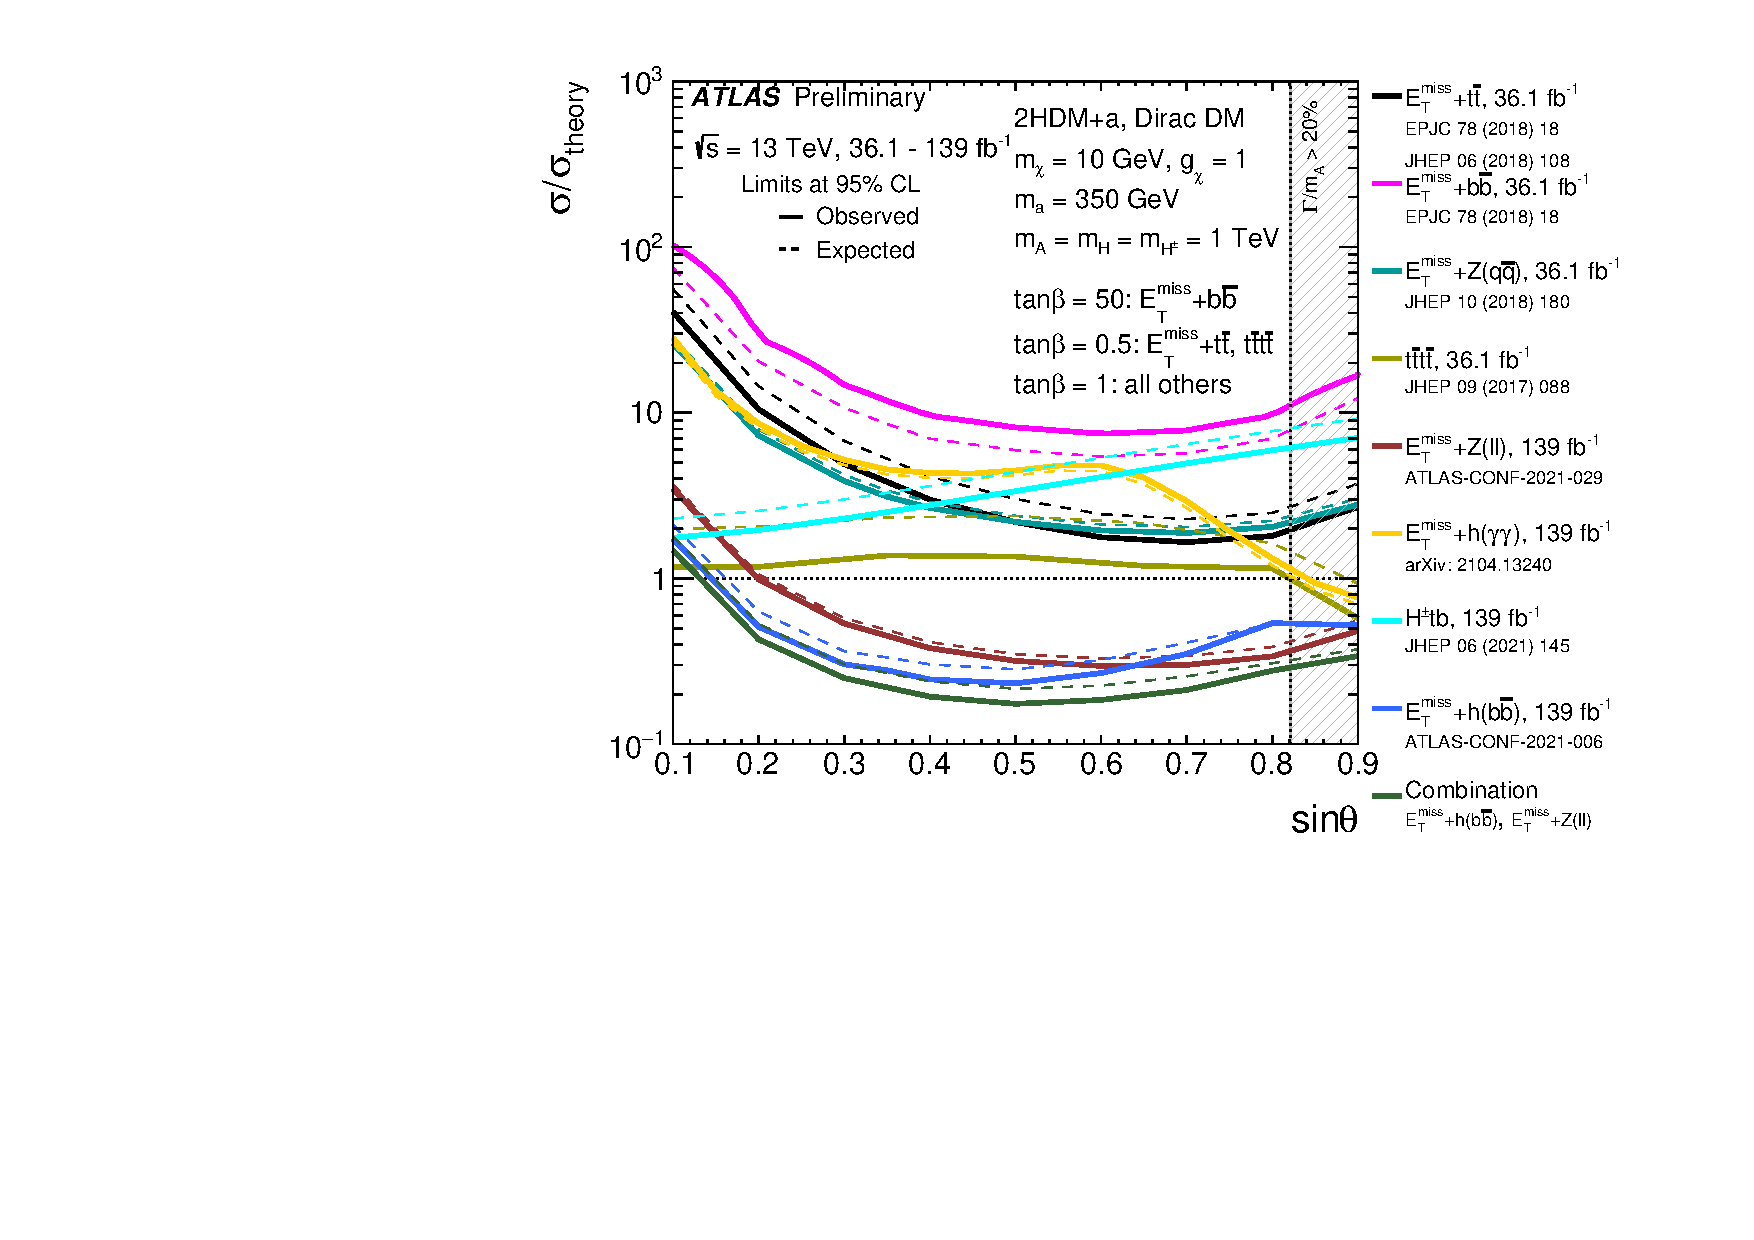
\includegraphics[width = 0.495\textwidth]{HPLUSTB/DM/sin_350_1000_1_10.pdf}
    \caption{Observed (solid lines) and expected (dashed lines) exclusion limits at 95\% CL for the 2HDM+a model as a function of $\sin\theta$ with $m_A = 600$~GeV, $m_a = 200$~GeV (left) and $m_A = 1$~TeV, $m_a = 350$~GeV (right). The results are shown for several individual searches as well as the combination of the $\MET+Z(\ell^+\ell^-)$ and $\MET+h(\bbar)$ searches.}
    \label{Hplustb:2HDMa_sintheta}
\end{figure}

Finally, the experimental reach of the different searches to the DM mass $m_\chi$ is shown in Figure~\ref{Hplustb:2HDMa_mchi}, which is the parameter with the strongest impact on the relic density predicted by the 2HDM+a. The searches are compared in terms of the observed exclusion limits on the ratio of the excluded cross-section to the nominal cross-section of the model as a function of $m_\chi$. For all signatures shown, the sensitivity is independent of $m_\chi$ as long as $m_a$ is allowed to decay into $\chi\bar{\chi}$. The strongest constraints are provided by the $\MET+ Z(\ell^+\ell^-)$ search. For higher DM masses, the sensitivity of the $\MET+X$ searches quickly decreases. For $m_\chi>m_a$/2, the strongest constraints are obtained from the $H^+$ search, which excludes the 2HDM+a for the chosen parameter values for all values $m_\chi$, as the production of the $H^+$ signal does not depend on this parameter.\\

\begin{figure}[htb]
    \RawFloats
    \centering
    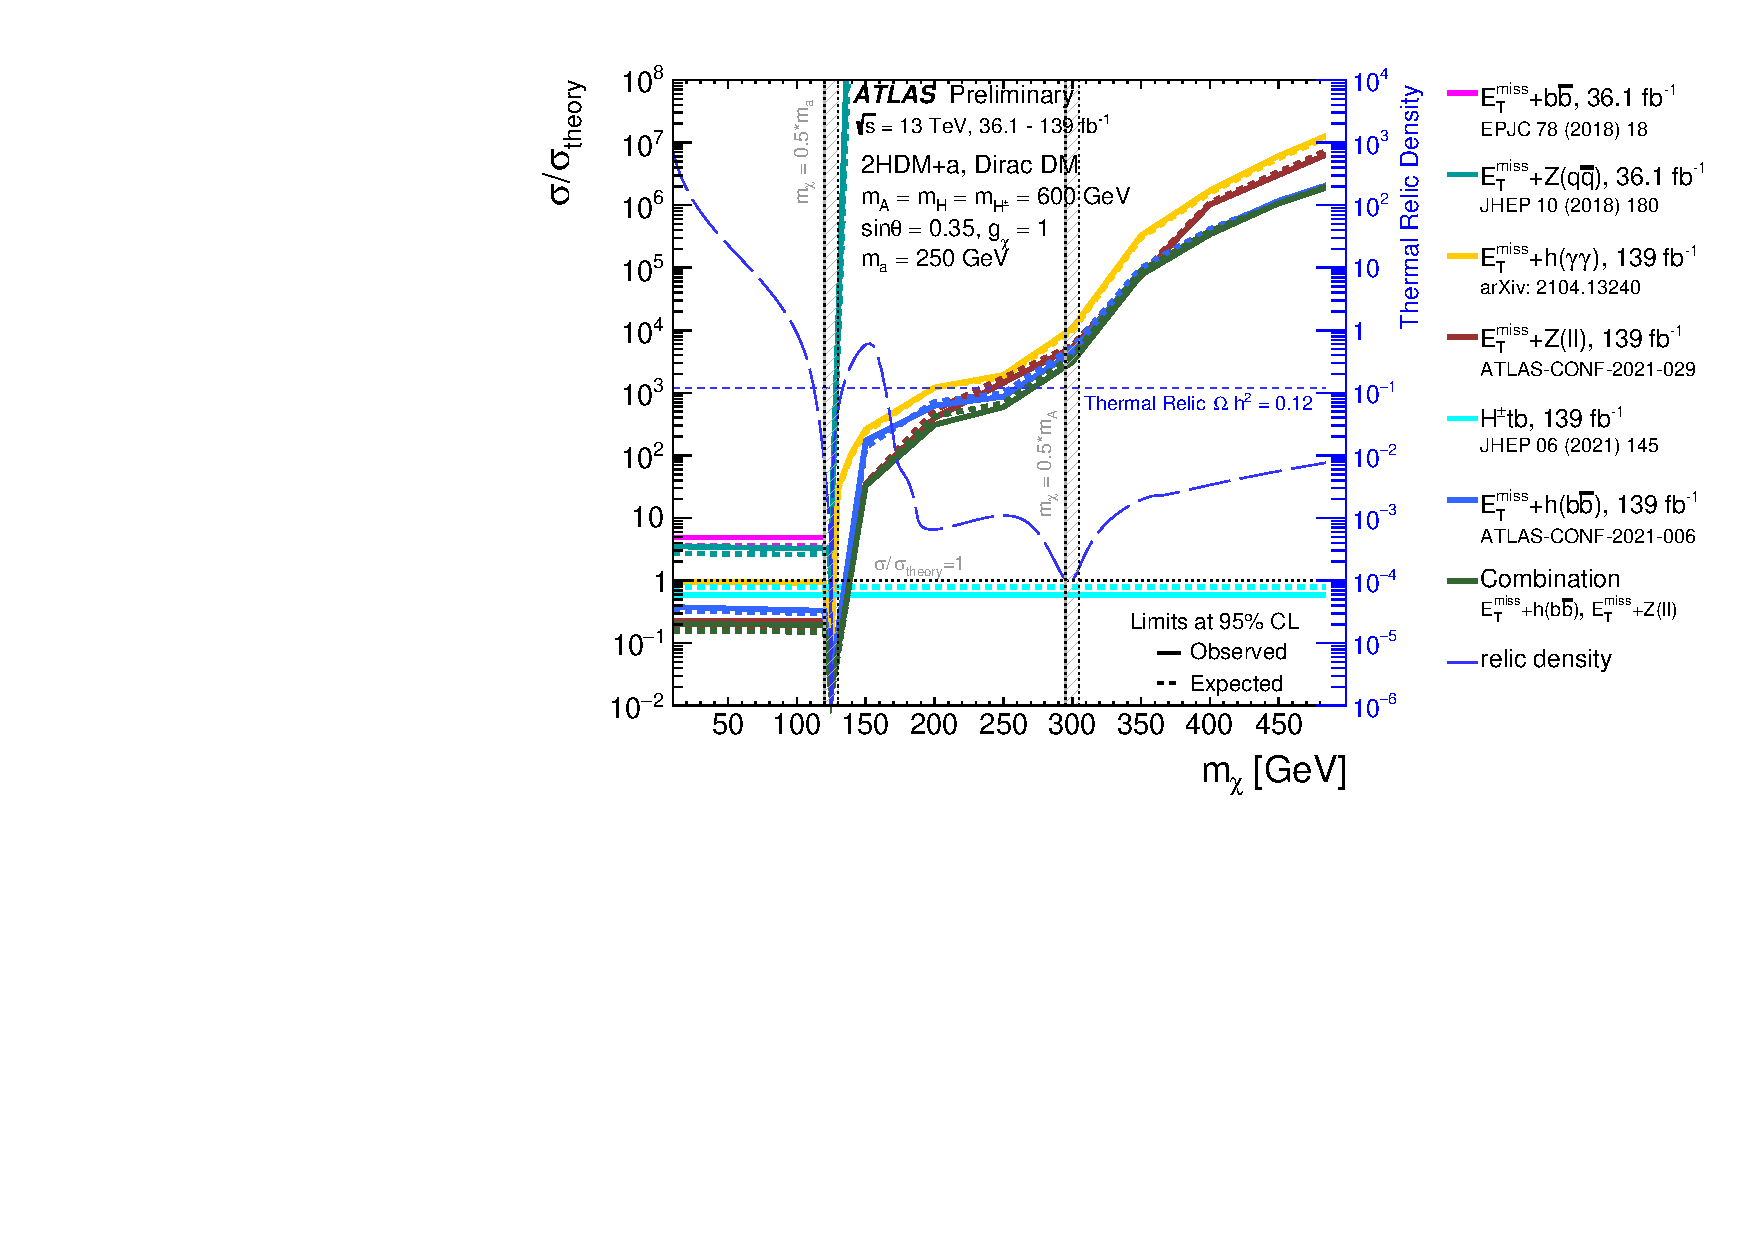
\includegraphics[width = 0.8\textwidth]{HPLUSTB/DM/mX_035_250_600.pdf}
    \caption{Observed (solid lines) and expected (dashed lines) exclusion limits for the 2HDM+a model as a function of $m_\chi$, following the parameter choices of $m_A = 600$~TeV, $m_a = 250$~GeV, $\tan\beta= 1.0$ and $\sin\theta=0.35$. The limits are calculated at 95\% CL and are expressed in terms of the ratio of the excluded cross-section to the nominal cross-section of the model. The results are shown for several individual searches as well as the combination of the $\MET+Z(\ell^+\ell^-)$ and $\MET+h(\bbar)$ searches. The relic density for each $m_\chi$ assumption is superimposed (long-dashed line) and described by the right vertical axis. The shaded region around 125 GeV indicates a $\pm$5 GeV band around the kinematic thresholds $m_\chi= 0.5 \cdot m_a$ and $m_\chi = 0.5 \cdot m_A$ where the generator
    results are deemed unreliable.}
    \label{Hplustb:2HDMa_mchi}
\end{figure}

% \section{Outlook}

% \begin{itemize}
%     \item Difficult to optimise 18 fits
%     \item Work on lowmass, decorrelate NP or reduce kttb correlation
%     \item Enchance selection with tigther btagging at low mass (less statistics at high mass)
%     \item new recommendations PFlow, b-tagging has improvements
%     \item Complement NN with low-level inputs (already tried to include alt samples in the training to reduce impact of sys)
%     \item Region definition and classification with other methods, like a reco NN, to enhance purity, explored in H+Wh
%     \item Include boosted ? dilepton ?
%     \item Estimate improvement for Run3?
% \end{itemize}


%The analysis strategy presented in the previous chapter was fxed before the start of the publication process and could not change afterwards, in order to proceed with the publication itself. The analysis development has however continued in view of the 100 fb1 of pp collisions that the LHC is expected to deliver by the end of Run-2. This chapter proposes a set of refnements that could be implemented to improve the sensitivity and robustness of the analysis. The frst part is dedicated to the low-mass region, with the aim of reducing the correlation between the signal and the ttb background, while the second part focuses on discrimination techniques. The conclusion provides the expected limit obtained with the proposed changes and the projection of such a limit to the integrated luminosity of 100 fb-1
%. All results are to be intended as preliminary.


% The ttHbb analysis presented in Chapters 13 and 14 is dominated by systematic uncertainties
% among which the modelling of the ttb background is by far the largest uncertainty. In the following, ideas to further reduce the systematic uncertainties and ideas to improve the general analysis strategy will be discussed. The multivariate techniques, namely the reconstruction and classification BDTs, are well suited to be replaced by Neural Networks opening new possibilities in the reconstruction and classification of events. And in particular, the improvements achieved within this thesis in the b-tagging algorithm performance described in detail in Part III are a great basis for further improvements. In the following two different optimisation possibilities are demonstrated: a new tagger incorporating the tt1B category and a first look into possible improvements using the newly optimised b-tagging algorithm DL1r